\documentclass{mcmthesis}
\mcmsetup{CTeX = false,    % 使用 CTeX 套装时,设置为 true
          tcn = {2429301}, problem = \textcolor{red}{C},
          sheet = true, titleinsheet = true, keywordsinsheet = true,
          titlepage = false, abstract = false}
        
\usepackage{newtxtext}     % \usepackage{palatino}
\usepackage[backend=bibtex]{biblatex}   % for RStudio Complie

\usepackage{tocloft}
\usepackage{graphicx} % 用于插图
\usepackage{subcaption} % 用于子图形

\setlength{\cftbeforesecskip}{6pt}
\renewcommand{\contentsname}{\hspace*{\fill}\Large\bfseries Contents \hspace*{\fill}}

\title{Research on the Impact of Player Momentum on Tennis Matches}
% \author{\small \href{http://www.latexstudio.net/}
%   {
\includegraphics[width=7cm]{mcmthesis-logo}}}
\date{\today}

\begin{document}

\begin{abstract}
    \qquad The 2023 Wimbledon Open highlighted Momentum's role in tennis, where Carlos's win over Djokovic demonstrated its impact on outcomes. Our study quantifies momentum to analyze its influence on match factors.

    In task 1, we developed a methodology to quantify the momentum of athletes in tennis matches, employing data cleaning, feature engineering, and machine learning models. This framework allows for the real-time tracking of momentum shifts, offering insights into performance dynamics at crucial moments. Our findings indicate that players with higher momentum scores are more likely to score in subsequent games, with the likelihood increasing as the momentum difference widens. Thus, athletes exhibiting greater momentum have a discernible advantage in performance. This concise approach integrates both our research method and conclusions, aiming for brevity and clarity in line with academic standards.

    In task 2, our methodology utilizes the ruptures Python library for time series change point detection, enabling the analysis of non-stationary signals through a variety of parametric and non-parametric models. This library, known for its robust offline detection capabilities, offers a user-friendly interface and modular design, facilitating the integration and expansion of algorithms within its framework.Our findings indicate that the streaks and turning points in an athlete's performance are not random, contradicting the coach's assertion.

    For Task 3 Long Short-Term Memory Model (LSTM) and Local Interpretable Model (LIME) were used to analyze and predict the fluctuation of athletes' momentum in tennis matches. By preprocessing the match data and selecting key factors such as first serve success rate, first serve scoring rate, second serve scoring rate, athlete running distance difference, serve side and score difference as feature inputs, the LSTM model was utilized to predict the changes in athlete momentum. The data and visualization images related to the model performance were obtained through model training, showing that the loss of the model on the training and test sets decreases with the increase of the training period, indicating that the predictive ability of the model improves over time. The mean absolute error (MAE) of the model was 1.0477, the mean square error (MSE) was 1.6303, and the root mean square error (RMSE) was 1.2768, and these metrics indicate that the model has some prediction accuracy.

    For Task 4 further used the LIME model to analyze the most important factors for the prediction of match momentum changes, and based on the results of these analyses, specific strategy recommendations were made for the athletes, including improving the first serve scoring rate, optimizing the second serve scoring rate, controlling the match tempo, and making comprehensive training and strategy adjustments. Through this combination of model analysis and strategy recommendations, the aim is to help athletes better understand momentum changes in matches and provide scientific data to support their future matches, thus significantly improving their game and chances of winning.
    \begin{keywords}
        Athlete Kinetic Energy, Change Point Detection, Runs Regression, LSTM, LIME
    \end{keywords}
\end{abstract}

\maketitle

%% Generate the Table of Contents, if it's needed.
% \renewcommand{\contentsname}{\centering Contents}
\tableofcontents   % 若不想要目录, 注释掉该句
\thispagestyle{empty}

\newpage


\section{Introduction}

\subsection{Background}
Tennis matches are often intense and fast-paced, and this is especially true of the competition between top professionals. In the men's final of the 2023 Wimbledon Open, where Carlos defeated Novak Djokovic to end a 13-year run, the ever-changing nature of the match brought the concept of Momentum back to the forefront of people's minds. Momentum is often viewed as the intangible force of momentum in a team's or individual's performance, which can be built up through a series of successful actions and can significantly affect the psychological and physical state of a match. This makes it possible for players with similar strengths to score points that do not necessarily follow the 50\% probability distribution, and for a seemingly dominant side to sometimes score consecutive points, or even to win consecutive sets in a fluctuating fashion, which is often attributed to "momentum". Therefore, it is very important for coaches to understand the "momentum" of their players and make appropriate instructions in competitive matches. In this context, we hope that through quantifiable data, coaches can better understand the real-time status of the players, so as to make more appropriate suggestions for the players.


\subsection{Literature Review}
\begin{itemize}


    \item[] {\bf Research on Vinicius Pradoda Fonseca} \\
        \hspace*{2em} Based on the data given in the question, and taking into account the factor of higher probability of winning for the serve side in a tennis match, a mathematical model was established to try to quantitatively analyze the momentum of the players in the match.

    \item[] {\bf Research by Helmut Dietl} \\
        \hspace*{2em} Research by Helmut Dietl further supports the importance of momentum in game predictions, particularly in the NHL and European soccer. By combining features of momentum and frequency, they proposed ways to improve pre-match prediction models. This comprehensive research approach is expected to provide a more comprehensive perspective for future sports science research and help deepen our understanding of the factors behind game outcomes.

    \item[] {\bf Research by Tracey M Covassin} \\
        \hspace*{2em} Tracey M Covassin's research focuses on the impact of players' psychological state on the results of tennis matches. By investigating factors such as emotional state, anxiety, self-confidence, triggering events and psychological motivation, they found that athletes with high self-confidence, low anxiety and low total emotional interference were more likely to achieve success. This provides empirical support for sports psychology, showing that an athlete's mental state before competition plays a key role in performance.

    \item[] {\bf Research by Yang Zhimin (2010)} \\
        \hspace*{2em} Yang Zhimin's research took tennis as the research object. Through detailed analysis of technical indicators, he determined the four factors that most affect the outcome of the game. First serve points scored, second serve points scored, first serve returned points scored, second serve returned points scored and backhand grip type are considered key factors. This not only provides clear guidance for training, requiring athletes to improve their serve and return scoring rates, but also emphasizes the decisive impact of technical details on the outcome of the game.

\end{itemize}

\begin{figure}[ht]
    \centering
    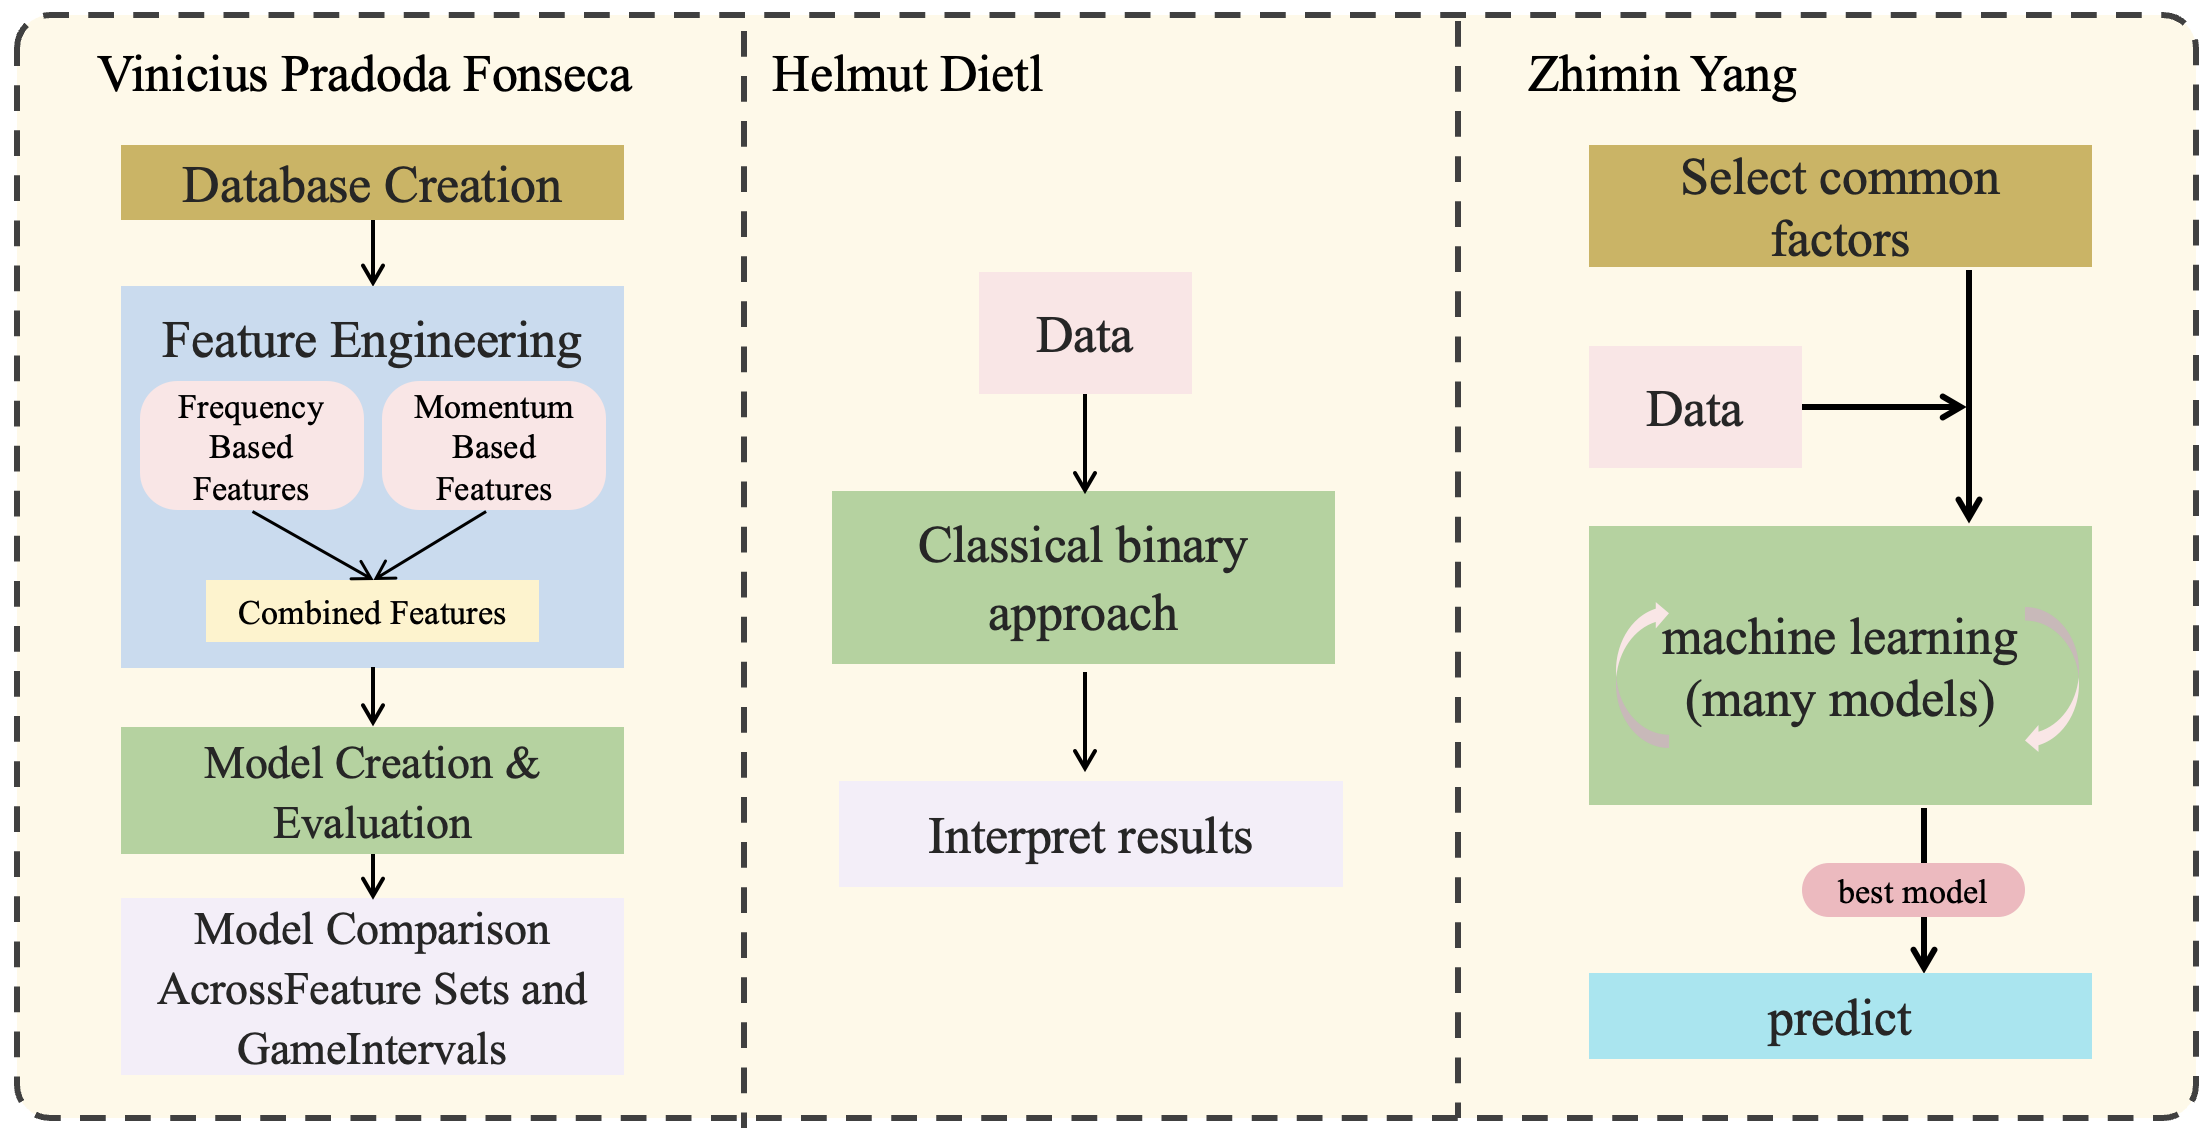
\includegraphics[width=\linewidth]{Literature Review.png} % 根据需要调整图片宽度
    \caption{Comparison of different data analysis approaches by Vinicius Pradoda Fonseca, Helmut Dietl, and Zhimin Yang.}
    \label{fig:literature_review}
\end{figure}

\subsection{Restatement of the Problem}
In this topic, we have detailed data based on men's singles matches after the first two rounds of the 2023 Wimbledon Open, which include match number, time of play, first serve scoring data, and type of winning shot. Based on this data, we will address the following task posed in the article by taking into account the advantageous factors of the server in conjunction with the flow of the match:

\begin{itemize}
    \item[] {\bf Task 1}: Based on the data given in the task, and taking into account the factor of higher probability of winning for the serve side in a tennis match, a mathematical model was established to try to quantitatively analyze the momentum of the players in the match.

    \item[] {\bf Task 2}: Using the model developed in Task 1, respond to the data or graphs to see if there is a pattern to the concept of momentum in the game. Attempt to empirically test the role of "momentum" in the game.

    \item[] {\bf Task 3}:
        \begin{itemize}
            \item[a)] Build a mathematical model that attempts to predict a player's future "momentum" using data from a single game.
            \item[b)] Identify factors in the game that may affect the player's "momentum" and make recommendations to the player based on those factors.
        \end{itemize}

    \item[] {\bf Task 4}: Attempt to apply the prediction model in Problem 3 to other matches, such as pool matches with similar rules to tennis, while introducing new factors such as court surfaces, different rules, etc., depending on the match. Reflect the prediction ability of the same model under different matches through data.

\end{itemize}
\newpage
\subsection{Our work}

    \begin{figure}[ht]
        \centering
        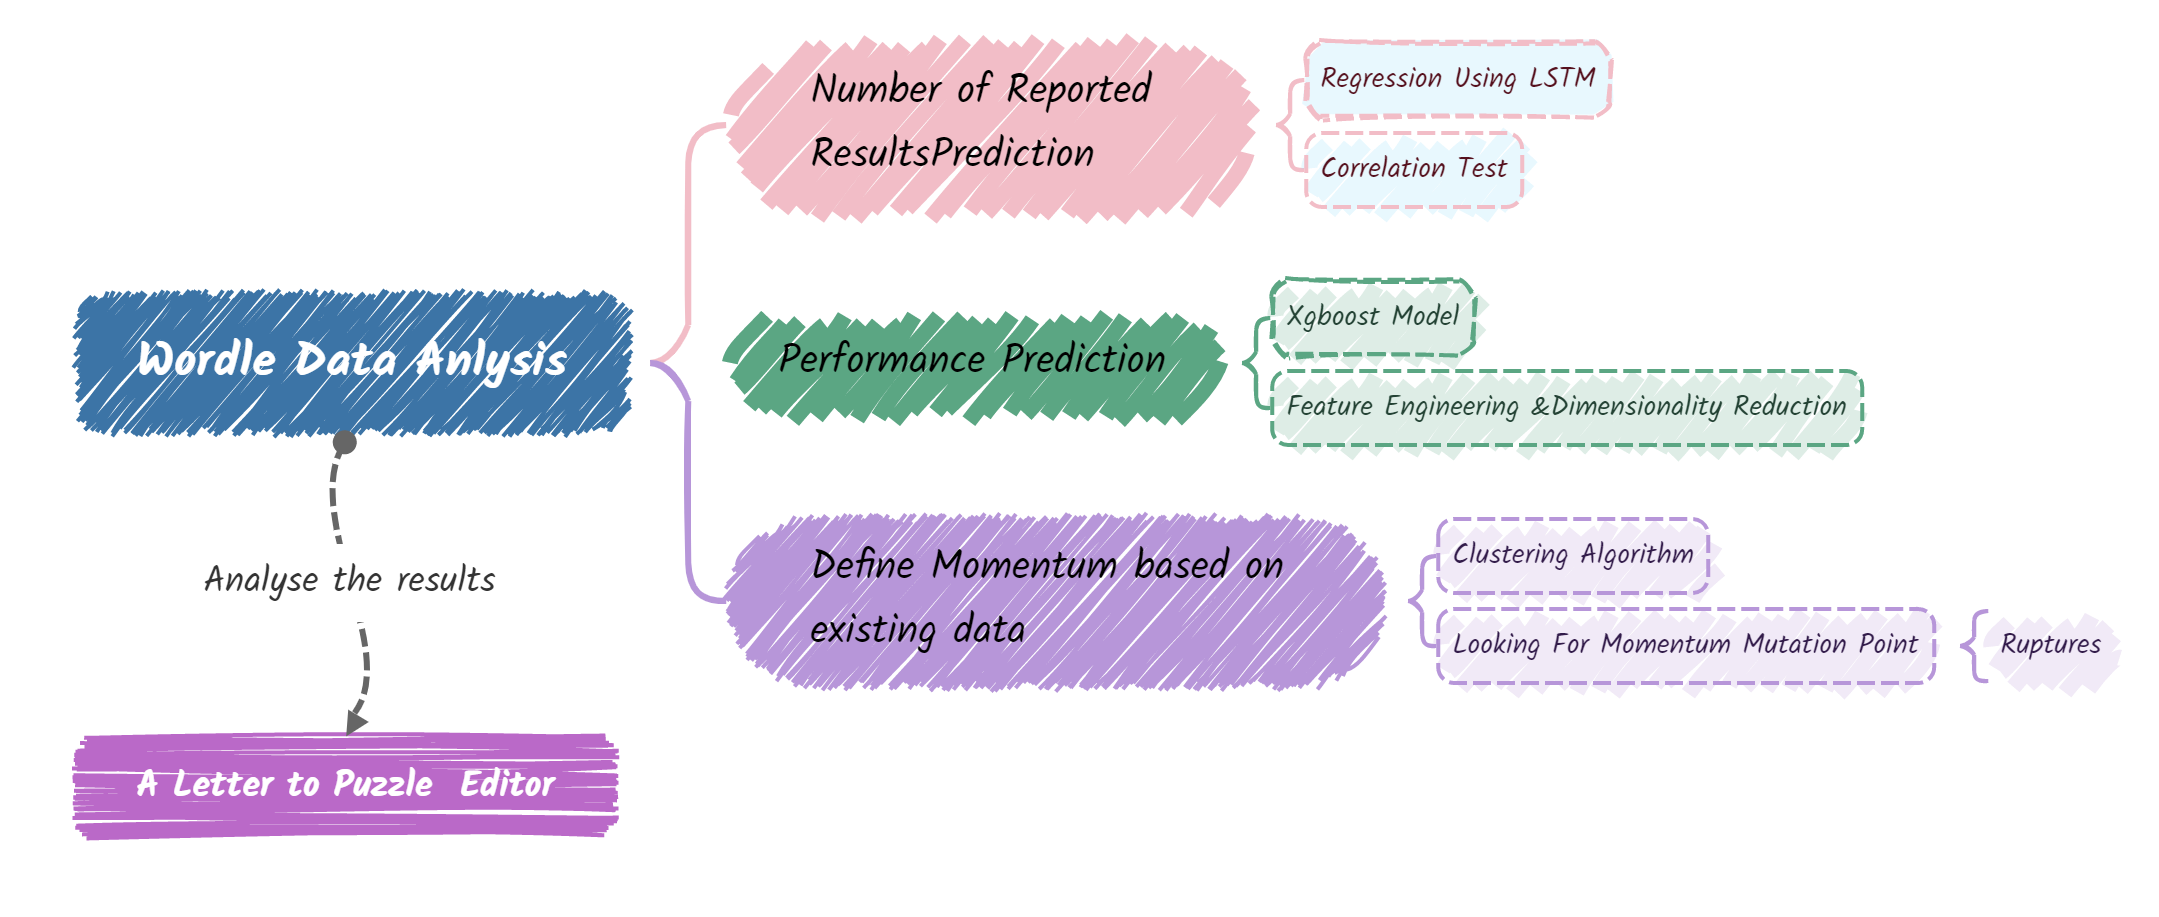
\includegraphics[width=\linewidth]{OurWork.jpg} % 根据需要调整图片宽度
        \caption{Comparison of different data analysis approaches by Vinicius Pradoda Fonseca, Helmut Dietl, and Zhimin Yang.}
        \label{fig:literature_review}
    \end{figure}
\newpage
\section{Assumptions and Justification}

In order to simplify the above problems, we make the following reasonable assumptions:

\begin{itemize}
    \item[] {\bf Assumption 1}: Assumed that the selected characteristics (e.g., number of aces, double faults, scoring rate, etc.) are representative of a player's performance in a match and the variation in momentum.

    \item[] {\bf Assumption 2}: Assumed that the serving team has a higher probability of winning each service game, i.e. the serving team usually has a greater advantage than the receiving team.

    \item[] {\bf Assumption 3}: Assume that different stages of the match (e.g., different sets and games) have different effects on a player's momentum. For example, a player's momentum may change more in the later stages of a match.

    \item[] {\bf Assumption 4}: To simplify the model, it is assumed that each point in the match is independent, i.e., a player's performance on each serve depends only on the current serve and is independent of previous points or the outcome of the game.

\end{itemize}

\section{Notations}


% \begin{center}
%     \begin{tabular}{clc}
%         {\bf Symbols} & {\bf Description}                    & \quad {\bf Unit}        \\[0.25cm]
%         $h$           & Convection heat transfer coefficient & \quad W/(m$^2 \cdot$ K)
%         \\[0.2cm]
%         $k$           & Thermal conductivity                 & \quad W/(m $\cdot$ K)   \\[0.2cm]
%         $c_p$         & Specific heat                        & \quad J/(kg $\cdot$ K)  \\[0.2cm]
%         $\rho$        & Density                              & \quad kg/m$^2$          \\[0.2cm]
%         $\delta$      & Thickness                            & \quad m                 \\[0.2cm]
%         $t$           & Temperature                          & \quad $^\circ$C, K      \\[0.2cm]
%         $\tau$        & Time                                 & \quad s, min, h         \\[0.2cm]
%         $q_m$         & Mass flow                            & \quad kg/s              \\[0.2cm]
%         $\Phi$        & Heat transfer power                  & \quad W                 \\[0.2cm]
%         $T$           & A period of time                     & \quad s, min, h         \\[0.2cm]
%         $V$           & Volume                               & \quad m$^3$, L          \\[0.2cm]
%         $M,\,m$       & Mass                                 & \quad kg                \\[0.2cm]
%         $A$           & Aera                                 & \quad m$^2$             \\[0.2cm]
%         $a,\,b,\,c$   & The size of a bathtub                & \quad m$^3$
%     \end{tabular}
% \end{center}

\begin{center}

    \begin{tabular}{clc}



        \textbf{Symbol} & \textbf{Description}                 & \textbf{Unit} \\ [0.25cm]



        \(C_t\)         & Cell state at time \(t\)             & N/A           \\ [0.25cm]

        \(h_t\)         & Hidden state at time \(t\)           & N/A           \\ [0.25cm]

        \(i_t\)         & Input gate activation at time \(t\)  & N/A           \\ [0.25cm]

        \(f_t\)         & Forget gate activation at time \(t\) & N/A           \\ [0.25cm]

        \(\tilde{C}_t\) & Candidate cell state at time \(t\)   & N/A           \\ [0.25cm]
    \end{tabular}

\end{center}

\noindent Where we define the main parameters while specific value of those parameters will be given later.

\section{Model Overview}

In our basic model, we aim at three goals: keeping the temperature as even as possible, making it close to the initial temperature and decreasing the water consumption.

We start with the simple sub-model where hot water is added constantly.
At first we introduce convection heat transfer control equations in rectangular coordinate system. Then we define the mean temperature of bath water.

Afterwards, we introduce Newton cooling formula to determine heat transfer
capacity. After deriving the value of parameters, we get calculating results via formula deduction and simulating results via CFD.

Secondly, we present the complicated sub-model in which hot water is
added discontinuously. We define an iteration consisting of two process:
heating and standby. As for heating process, we derive control equations and boundary conditions. As for standby process, considering energy conservation law, we deduce the relationship of total heat dissipating capacity and time.

Then we determine the time and amount of added hot water. After deriving the value of parameters, we get calculating results via formula deduction and simulating results via CFD.

At last, we define two criteria to evaluate those two ways of adding hot water. Then we propose optimal strategy for the user in a bathtub.
The whole modeling process can be shown as follows.

\section{Task 1: Identify superior player and visualize match flow}
Initially, our study focused on analyzing and constructing metrics to assess the game momentum of athletes, involving comprehensive data cleaning and feature engineering processes tailored to this objective. Following this, we harnessed machine learning models to develop a framework capable of measuring the momentum changes of athletes in real-time for each scored point. This methodology enables the evaluation of superior athlete performance at specific instances within the match.

\begin{figure}[h]
    \centering
    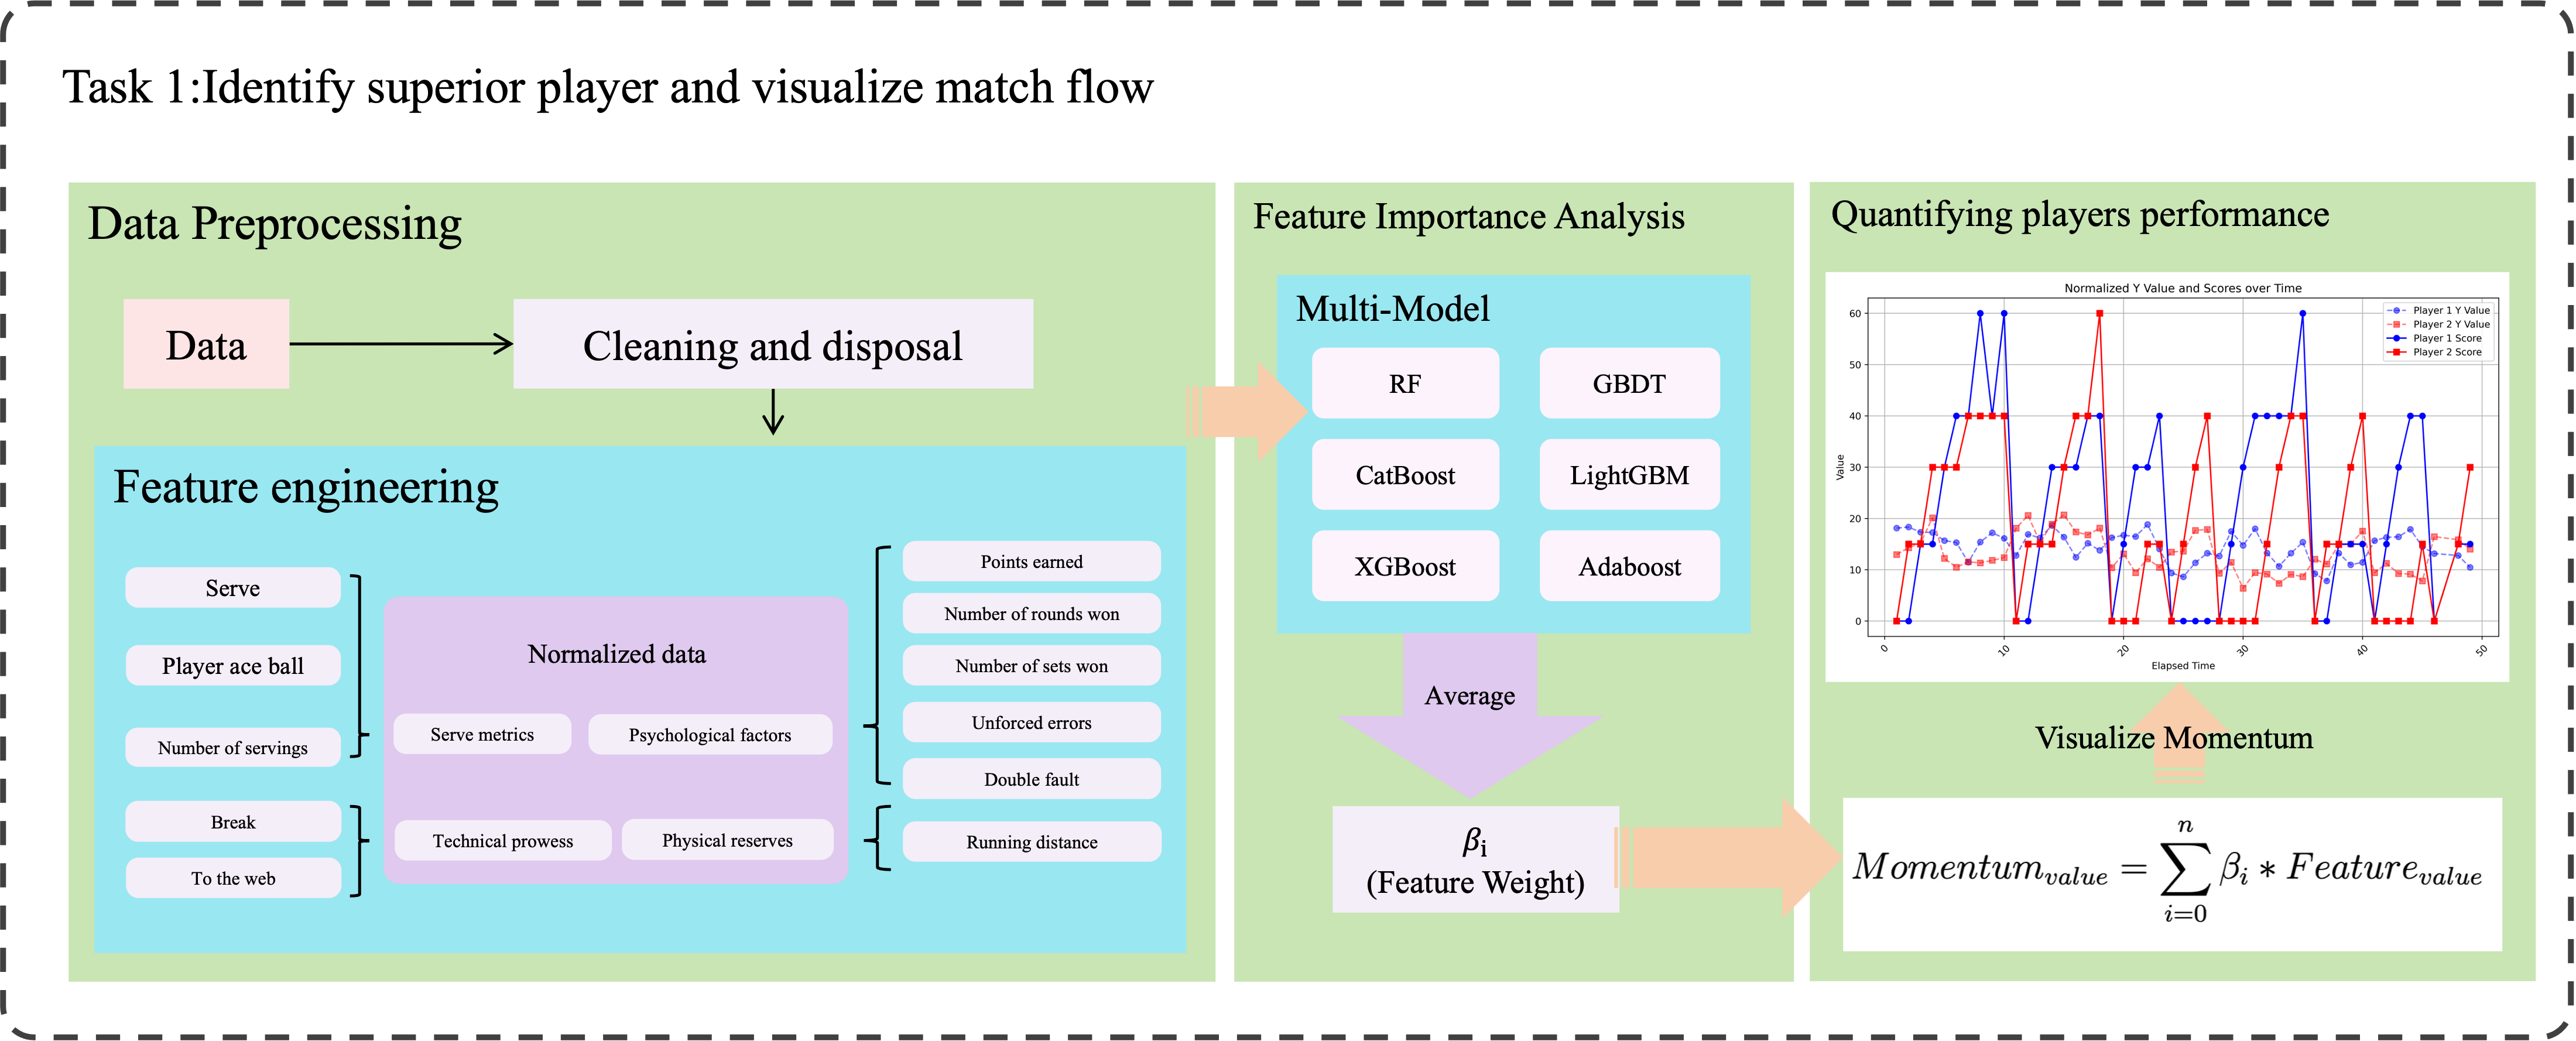
\includegraphics[width=16cm]{task1_总流程图.png}
    \caption{Task1 solution flow chart} \label{fig1}
\end{figure}

Subsequently, we leveraged this model to calculate the momentum values for each point scored by athletes throughout the competition. We then proceeded to create visual representations of the match progression based on these momentum calculations. This visualization aids in providing a clear and intuitive understanding of the match trends, enhancing the spectator's ability to discern the dynamics of the competition effectively.
\subsection{Data Preprocessing}
\subsubsection{Data Cleaning}
\qquad In the process of data handling and analysis, the treatment of missing and outlier values is crucial. This concerns not only the quality of the data but also directly impacts the accuracy of subsequent analytical outcomes. To reduce the computational complexity of subsequent data analysis and modeling, we performed preprocessing on the data provided in the attachment.
\begin{itemize}
    \item \textbf{Missing Value Detection}: We conducted missing value checks across all column features and opted to delete rows containing null values.
          It is noteworthy that a significant number of missing values were found in the return\_depth column. However, considering these missing values might result from service faults, we refrained from applying the aforementioned deletion operation to rows with null values in this particular column.
    \item {\bf Outlier Detection}: We employed the 3-sigma rule for independent outlier detection across all features and did not identify any outliers, inicating the data provided in the attachment is relatively clean.
\end{itemize}

\subsubsection{Momentum Feature Engineering}
\begin{figure}[h]
    \centering
    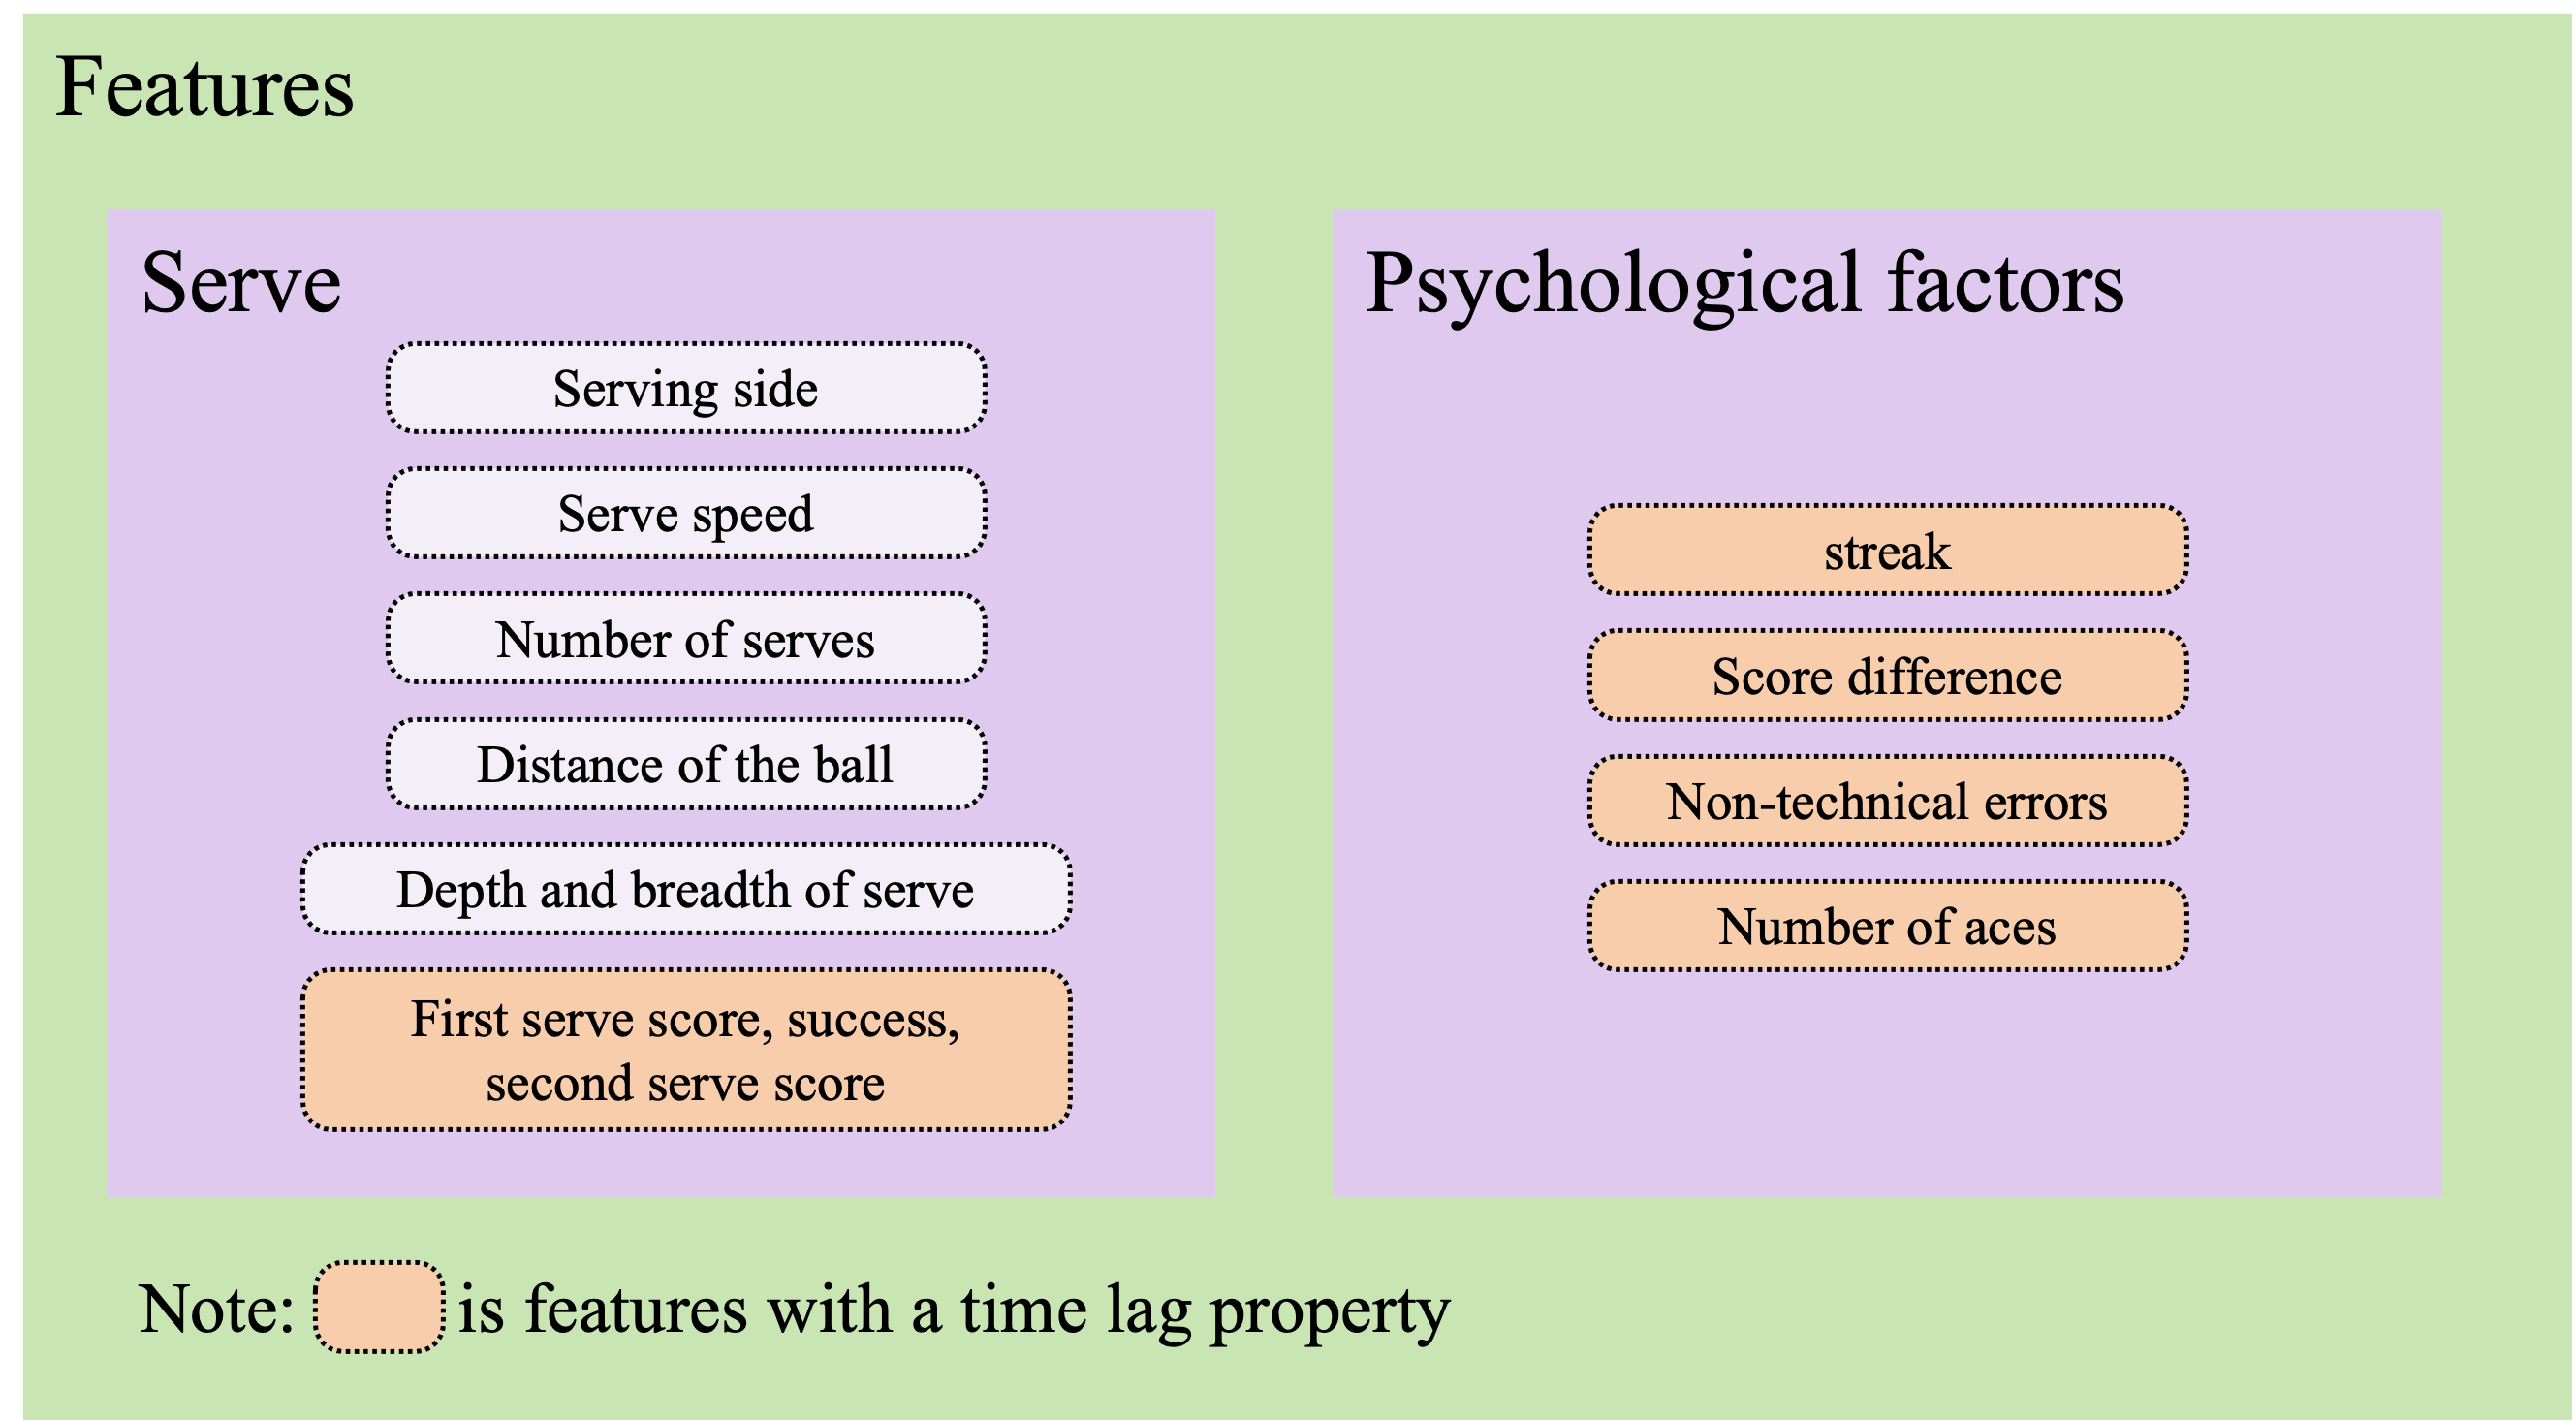
\includegraphics[width=14cm]{task1_特征图.png}
    \caption{Player performance evaluation indicators} \label{fig_img2}
\end{figure}

\qquad In tennis matches, an athlete's performance is not solely reflected in the basic score but involves multiple aspects, including technical skills, psychological resilience, tactics, and in-match proactivity. To provide a more comprehensive and nuanced evaluation system, thereby better understanding and analyzing an athlete's performance during matches, constructing new features is crucial. The following is an explanation and elaboration on the necessity of constructing these features and how they can aid in a deeper analysis of an athlete's match performance. Refer to Figure \ref{fig_img2} for a detailed indicator classification.
\begin{itemize}
    \item {\bf{First Serve Success Rate}}: The first serve is a key component in gaining an advantage in tennis matches, and the first serve success rate is directly linked to the ability to control the game. A high first serve success rate usually indicates that the player has an advantage in the serving phase, increasing the likelihood of scoring points in service games.
          \begin{equation} \label{eq1}
              % Momentum_{value} = \sum_{i=0}^n{\beta_i * Feature_{value}}
              First Serve Success Rate = \frac{Number of Successful First Serves}{Total First Serves Attempted} \times 100\%
          \end{equation}
    \item {\bf First Serve Points Won}: This metric further refines the analysis of the first serve success rate by not only focusing on whether the first serve is successful but also if it results in points won. It reflects the quality of the first serve and the player's ability to capitalize on the initiative gained from a successful first serve.
          \begin{equation} \label{eq1}
              First Serve Points Won = \frac{Points Won on First Serve}{Number of Successful First Serves} \times 100\%
          \end{equation}
    \item {\bf Second Serve Points Won}: Given that the second serve typically adopts a more conservative strategy, the second serve points won rate reflects the player's stability and adaptability in less favorable situations. This metric helps assess the player's performance following a first serve fault.
          \begin{equation} \label{eq1}
              Second Serve Points Won = \frac{Points Won on Second Serve}{Number of Successful Second Serves} \times 100\%
          \end{equation}
    \item {\bf Consecutive Points Won}: The number of consecutive points won demonstrates the player's ability to win points successively in a match, which is indicative of both technical and tactical prowess, as well as psychological dominance and the ability to manage pressure during the match.
    \item {\bf Points Difference}: The point difference can intuitively reflect the intensity of the match and the comparative strength of the opponents. A player's performance under different points differences can reveal their psychological stability and ability to adjust strategies under pressure.
          \begin{equation} \label{eq1}
              Points Difference = Player1's Points - Player2's Points
          \end{equation}
    \item {\bf Unforced Errors (within three points)}: Unforced errors, due to poor strategic choices or psychological factors rather than technical mishaps, help evaluate a player's decision-making ability and mental state during the match.
    \item {\bf Ace Count (within three points)}: An ace, a serve that results directly in a point without the opponent being able to touch the ball, reflects the precision and power of a player's serve. The number of aces is an important indicator of serving advantage.
\end{itemize}

\subsection{Multi-Model Feature Importance Analysis}
In order to quantify the effects of diverse indicators on player momentum, our approach leveraged machine learning classification algorithms to evaluate the contributions of various features towards the dependent variable. This method involved the application of several classification models to both identify and quantify the significance of these features accurately.

Subsequently, an integrated analysis was conducted by synthesizing the outputs from these models via a weighted average, culminating in the development of a comprehensive indicator.

This composite indicator aims to encapsulate the weighted contributions of each feature towards the dependent variable, thereby offering a nuanced understanding of their impact. The contributions of different features under various models are detailed in Table \ref{table:Feature importance in different models}, while Table \ref{table:5_2} outlines the performance metrics of these models.
\begin{table}[h!]
    \centering
    \caption{Feature importance in different models}
    \resizebox{\textwidth}{!}{%
        \begin{tabular}{lcccccc}
            \hline
            \textbf{Feature}                & \textbf{RF} & \textbf{Adaboost} & \textbf{GBDT} & \textbf{CatBoost} & \textbf{XGBoost} & \textbf{LightGBM} \\
            \hline
            server                          & 37.60\%     & 4.00\%            & 20.90\%       & 17.90\%           & 28.80\%          & 2.90\%            \\
            Players run distance difference & 7.20\%      & 7.00\%            & 11.20\%       & 6.00\%            & 3.60\%           & 11.40\%           \\
            p1 unf err count2r              & 8.00\%      & 3.00\%            & 6.90\%        & 6.30\%            & 10.30\%          & 4.10\%            \\
            speed mph                       & 5.60\%      & 4.00\%            & 6.60\%        & 6.50\%            & 2.20\%           & 10.60\%           \\
            p2 unf err count2r              & 7.50\%      & 3.00\%            & 6.50\%        & 7.80\%            & 9.30\%           & 3.30\%            \\
            p1 2nd serve win ratio          & 3.20\%      & 4.00\%            & 6.10\%        & 5.00\%            & 3.30\%           & 7.10\%            \\
            p2 1st serve win ratio          & 2.90\%      & 12.00\%           & 5.70\%        & 3.60\%            & 2.70\%           & 8.70\%            \\
            p1 1st serve win ratio          & 2.60\%      & 14.00\%           & 5.30\%        & 5.30\%            & 3.30\%           & 8.80\%            \\
            p2 2nd serve win ratio          & 3.10\%      & 10.00\%           & 5.20\%        & 4.50\%            & 2.80\%           & 5.90\%            \\
            p2 1st serve success ratio      & 1.90\%      & 15.00\%           & 5.00\%        & 3.90\%            & 3.10\%           & 7.80\%            \\
            p1 1st serve success ratio      & 1.80\%      & 10.00\%           & 4.80\%        & 6.00\%            & 3.30\%           & 8.20\%            \\
            Player score margin             & 1.60\%      & 3.00\%            & 4.00\%        & 3.90\%            & 2.70\%           & 6.50\%            \\
            continuous wins p1              & 2.40\%      & 3.00\%            & 3.50\%        & 6.00\%            & 5.10\%           & 4.00\%            \\
            continuous wins p2              & 3.00\%      & 5.00\%            & 2.80\%        & 6.40\%            & 5.10\%           & 3.00\%            \\
            serve width                     & 1.80\%      & 0.00\%            & 2.30\%        & 3.40\%            & 2.30\%           & 3.10\%            \\
            serve no                        & 2.90\%      & 0.00\%            & 1.00\%        & 2.90\%            & 5.20\%           & 1.50\%            \\
            p2 ace count2r                  & 3.60\%      & 1.00\%            & 1.00\%        & 1.50\%            & 3.70\%           & 1.10\%            \\
            serve depth                     & 0.90\%      & 1.00\%            & 0.80\%        & 1.20\%            & 1.50\%           & 1.30\%            \\
            p1 ace count2r                  & 2.40\%      & 1.00\%            & 0.40\%        & 1.90\%            & 1.90\%           & 0.90\%            \\
            \hline
        \end{tabular}
    }
    \label{table:Feature importance in different models}
\end{table}
The table showcases the performance of several machine learning models across various datasets, with a special focus on Accuracy and Precision (Recall and F1 Score can be considered as measures contributing to the overall precision and accuracy in the context of classification tasks). The models under consideration are LightGBM, CatBoost, AdaBoost, GBDT, and Random Forest.

These observations suggest that LightGBM and CatBoost, in particular, possess superior learning capabilities, as evidenced by their high accuracy rates on the training data. The slight decrease in accuracy on unseen data for these models indicates a potential for further refinement to enhance generalization without significantly compromising their inherent strengths. AdaBoost, GBDT, and Random Forest, with their consistent and balanced accuracy figures, underscore the robustness of these models in handling varied data scenarios.

Overall the performance metrics of LightGBM, CatBoost, AdaBoost, GBDT, and Random Forest models not only demonstrate their respective strengths in learning from training data but also provide a foundational understanding of their capability to discern and utilize the most impactful features for prediction. This intrinsic ability is crucial for leveraging feature importance to construct a weighted model that optimizes predictive accuracy and insight into the driving factors behind the model's decisions.
\begin{table}[htbp]
    \centering
    \caption{Model Performance Metrics}
    \begin{tabular}{@{}llllll@{}}
        \toprule
        \textbf{Model}                 & \textbf{Dataset}     & \textbf{Accuracy} & \textbf{Recall Rate} & \textbf{F1} & \\ \midrule
        \multirow{3}{*}{LightGBM}      & Training Set         & 0.896             & 0.896                & 0.896       & \\
                                       & Cross Validation Set & 0.711             & 0.711                & 0.711       & \\
                                       & Test Set             & 0.730             & 0.730                & 0.730       & \\
        \midrule
        \multirow{2}{*}{CatBoost}      & Training Set         & 0.902             & 0.902                & 0.902       & \\
                                       & Test Set             & 0.716             & 0.716                & 0.716       & \\
        \midrule
        \multirow{3}{*}{Adaboost}      & Training Set         & 0.717             & 0.717                & 0.717       & \\
                                       & Cross Validation Set & 0.701             & 0.701                & 0.701       & \\
                                       & Test Set             & 0.682             & 0.682                & 0.682       & \\
        \midrule
        \multirow{2}{*}{GBDT}          & Training Set         & 0.960             & 0.960                & 0.960       & \\
                                       & Test Set             & 0.703             & 0.703                & 0.703       & \\
        \midrule
        \multirow{3}{*}{Random Forest} & Training Set         & 0.747             & 0.747                & 0.747       & \\
                                       & Cross Validation Set & 0.714             & 0.714                & 0.714       & \\
                                       & Test Set             & 0.714             & 0.714                & 0.714       & \\
        \bottomrule
    \end{tabular}\label{table:5_2}
\end{table}

\subsection{Building Dynamic Momentum Index Model}
Table \ref{table:updated_multi_model_feature_importance_analysis} demonstrates the importance of the contributions to the dependent variable, as determined by averaged weights. Leveraging this analytical framework, we formulated a model to assess momentum, detailed in the specified formula \ref{eq:momentum_calculation_formula}.
\begin{table}[h!]
    \centering
    \caption{Multi-Model Feature Importance Analysis}
    \begin{tabular}{lcc}
        \hline
        \textbf{Feature}                & \textbf{Feature symbols} & \textbf{AVG weigh} \\
        \hline
        server                          & \(x_1\)                  & 18.68\%            \\
        Players run distance difference & \(x_2\)                  & 7.73\%             \\
        p1 unf err count2r              & \(x_3\)                  & 6.43\%             \\
        speed mph                       & \(x_4\)                  & 5.92\%             \\
        p2 unf err count2r              & \(x_5\)                  & 6.23\%             \\
        p1 2nd serve win ratio          & \(x_6\)                  & 4.78\%             \\
        p2 1st serve win ratio          & \(x_7\)                  & 5.93\%             \\
        p1 1st serve win ratio          & \(x_8\)                  & 6.55\%             \\
        p2 2nd serve win ratio          & \(x_9\)                  & 5.25\%             \\
        p2 1st serve success ratio      & \(x_{10}\)               & 6.12\%             \\
        p1 1st serve success ratio      & \(x_{11}\)               & 5.68\%             \\
        Player score margin             & \(x_{12}\)               & 3.62\%             \\
        continuous wins p1              & \(x_{13}\)               & 4.00\%             \\
        continuous wins p2              & \(x_{14}\)               & 4.22\%             \\
        serve width                     & \(x_{15}\)               & 2.15\%             \\
        serve no                        & \(x_{16}\)               & 2.25\%             \\
        p2 ace count2r                  & \(x_{17}\)               & 1.98\%             \\
        serve depth                     & \(x_{18}\)               & 1.12\%             \\
        p1 ace count2r                  & \(x_{19}\)               & 1.42\%             \\
        \hline
    \end{tabular}
    \label{table:updated_multi_model_feature_importance_analysis}
\end{table}
\begin{equation} \label{eq:momentum_calculation_formula}
    Momentum_{value} = \sum_{i=0}^n{\beta_{i} * Feature_{value}}
\end{equation}

\subsection{Dynamic Momentum Index-Driven Visualization of Match Flow}
% 我们通过上述公式 \ref{eq:动量计算公式}计算出每一个Point中运动员的势头变化情况.
% 选手的势头被视为是一个由多个纬度特征整合而成的一个线性模型。
% 我们随后将结合比赛的流程进行来可视化选手的表现,选取了“2023-wimbledon-1301”场次的对模型进行可视化分析和说明。
% 如图1所示,我们可以看到选手的势头在几分中都会出现强烈的波动,这能反映出选手的得分的概率在每一分之间迅速变化。
% 由于在特征工程阶段,我们加入了一些带有时间滞后属性的特征,例如一发得分率、一发成功率、近几回合的ace球数等等,因此这个Dynamic Momentum Index模型也能捕捉到玩家的一些过往的表现,这同样是符合我们日常比赛的逻辑直觉的。
We calculated the momentum change of each athlete in every Point using the formula referred to as \ref{eq:momentum_calculation_formula}. The athlete's momentum is considered to be a linear model integrated from multiple dimensional features. Subsequently, we combined the match process for visualizing the athlete's performance, selecting the "2023-wimbledon-1301" match for visualization analysis and explanation. As shown in Figure 1, we can observe significant fluctuations in the athlete's momentum within minutes, reflecting the rapid changes in the probability of scoring between each point. Due to the inclusion of features with time-lag attributes during the feature engineering stage, such as first serve score rate, first serve success rate, and the number of aces in recent rounds, the Dynamic Momentum Index model can also capture some of the player's past performances, aligning with our logical intuition of match dynamics.

\begin{figure}[h]
    \centering
    \begin{minipage}{0.5\textwidth}
        \centering
        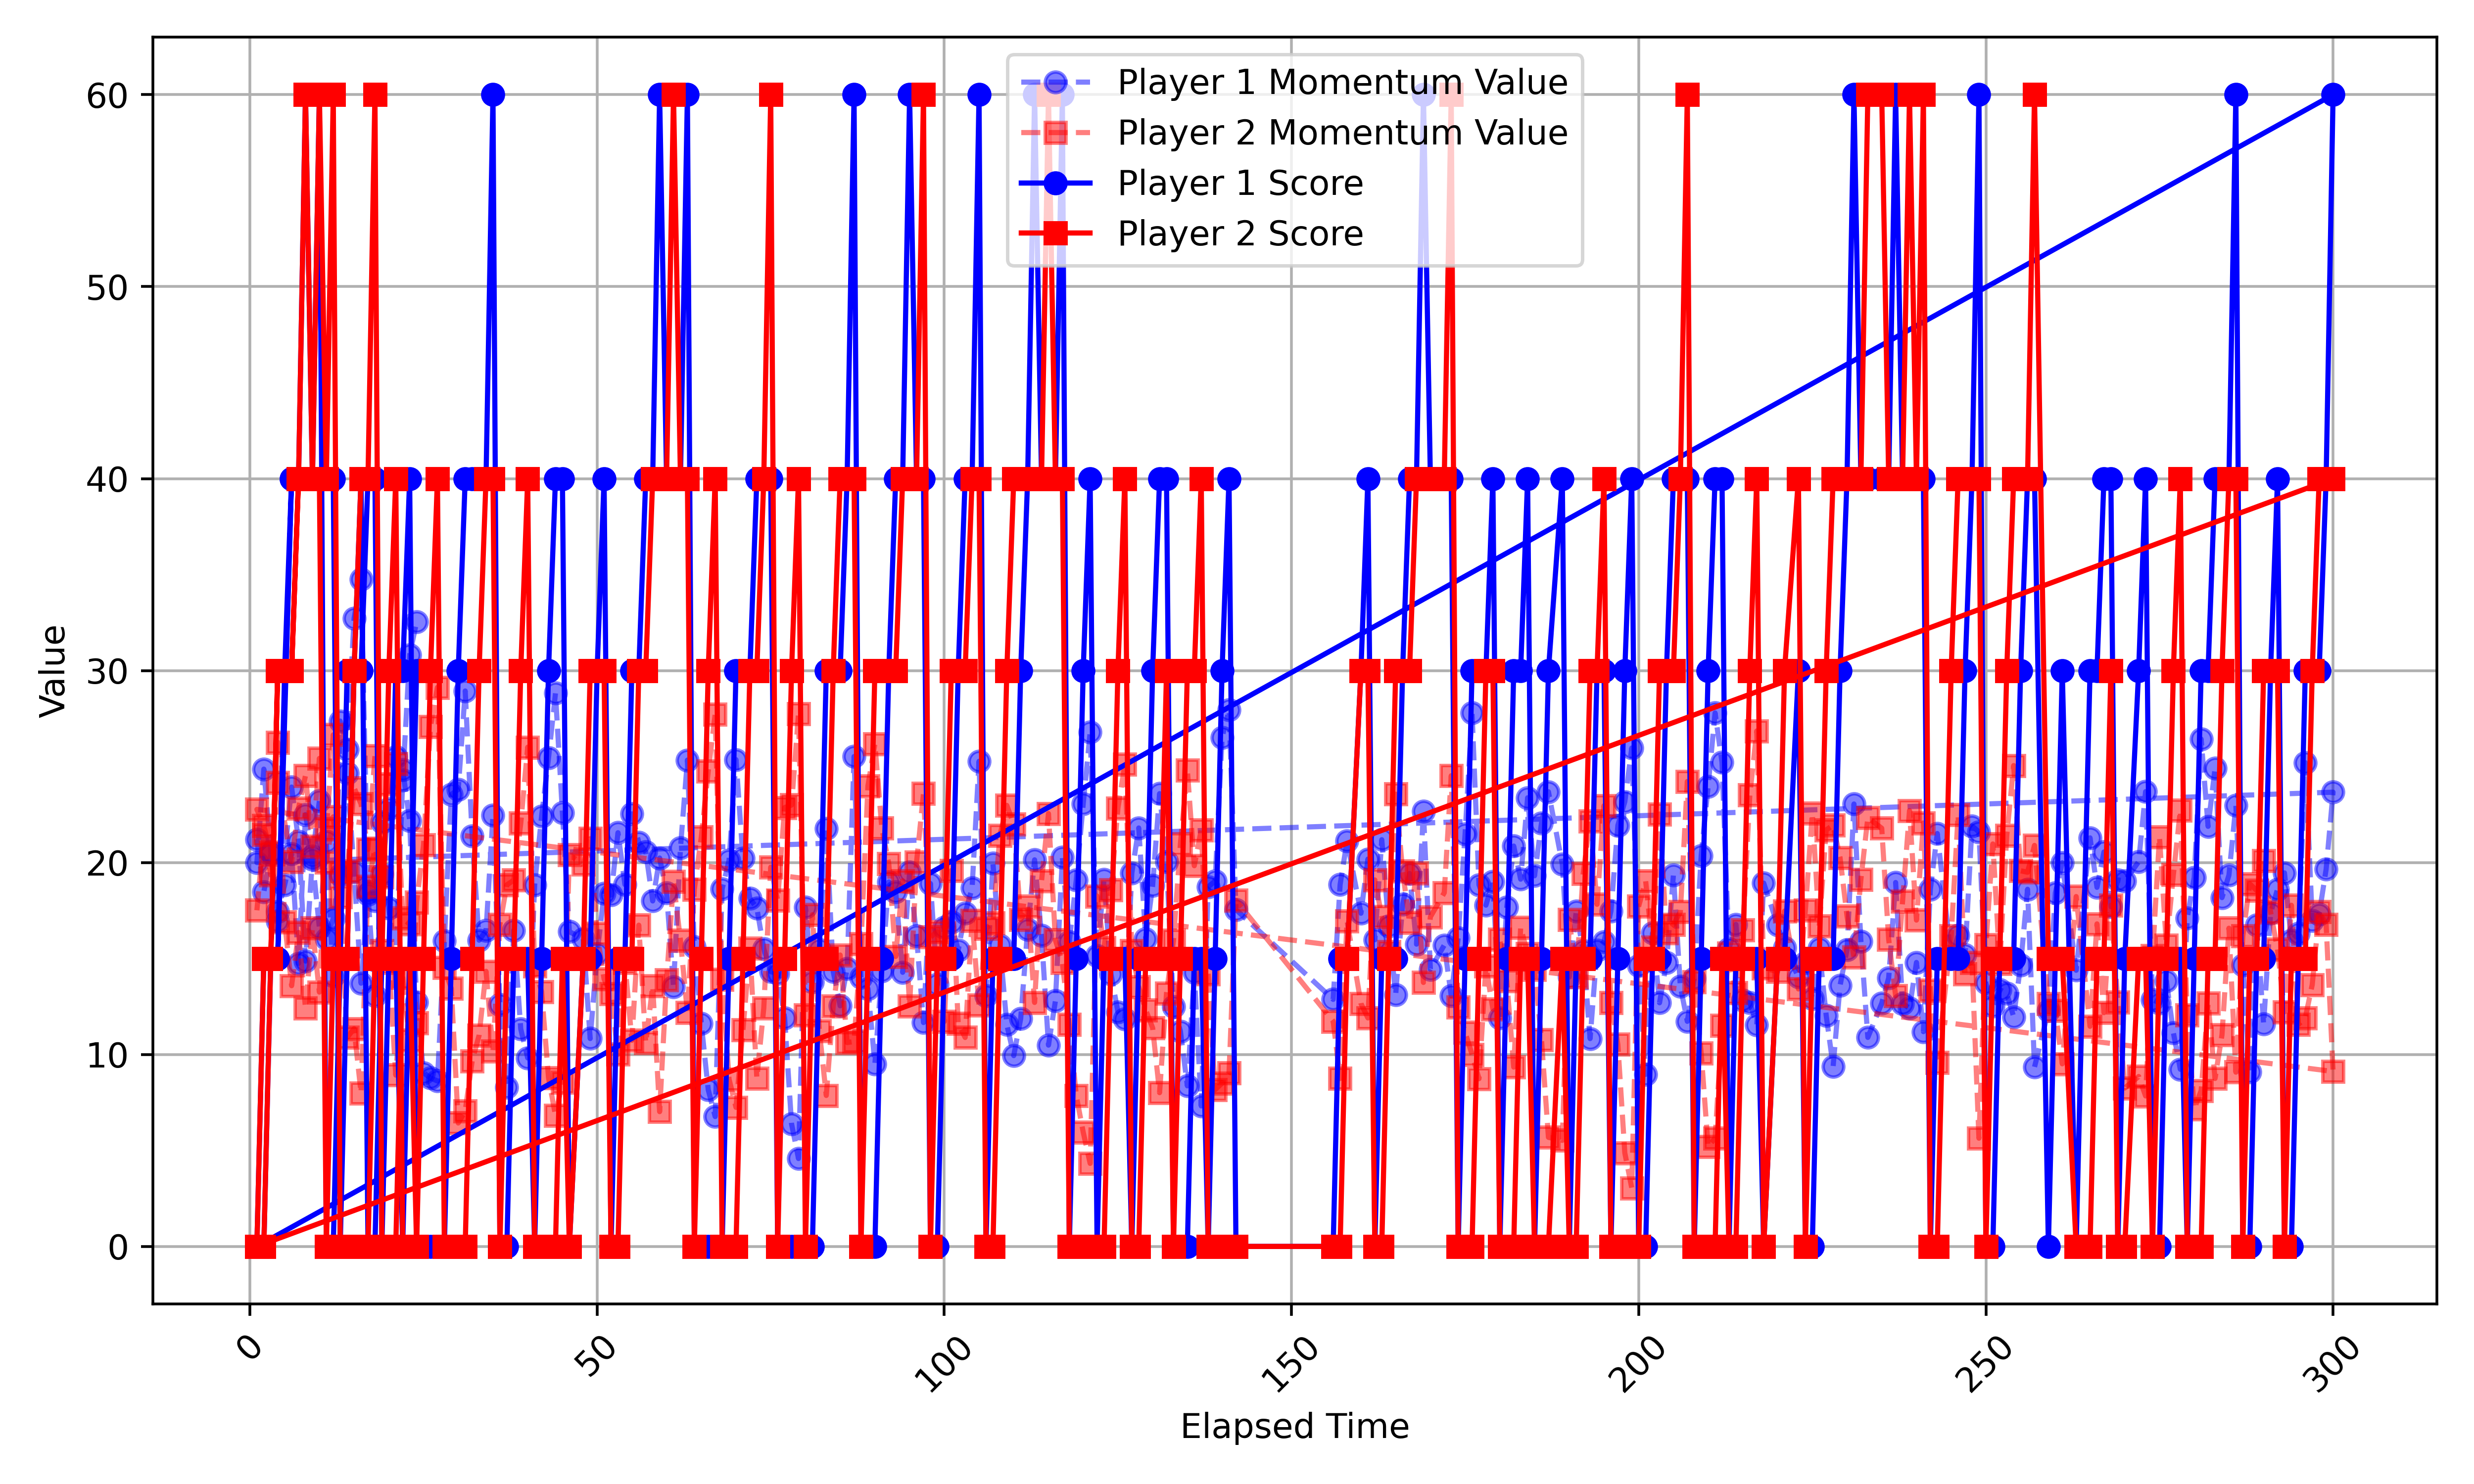
\includegraphics[width=\linewidth]{q11/动量_比赛.png} % 调整图像宽度以适应minipage宽度
        \caption{Game flow chart}
        \label{fig_q11_1}
    \end{minipage}\hfill
    \begin{minipage}{0.5\textwidth}
        \centering
        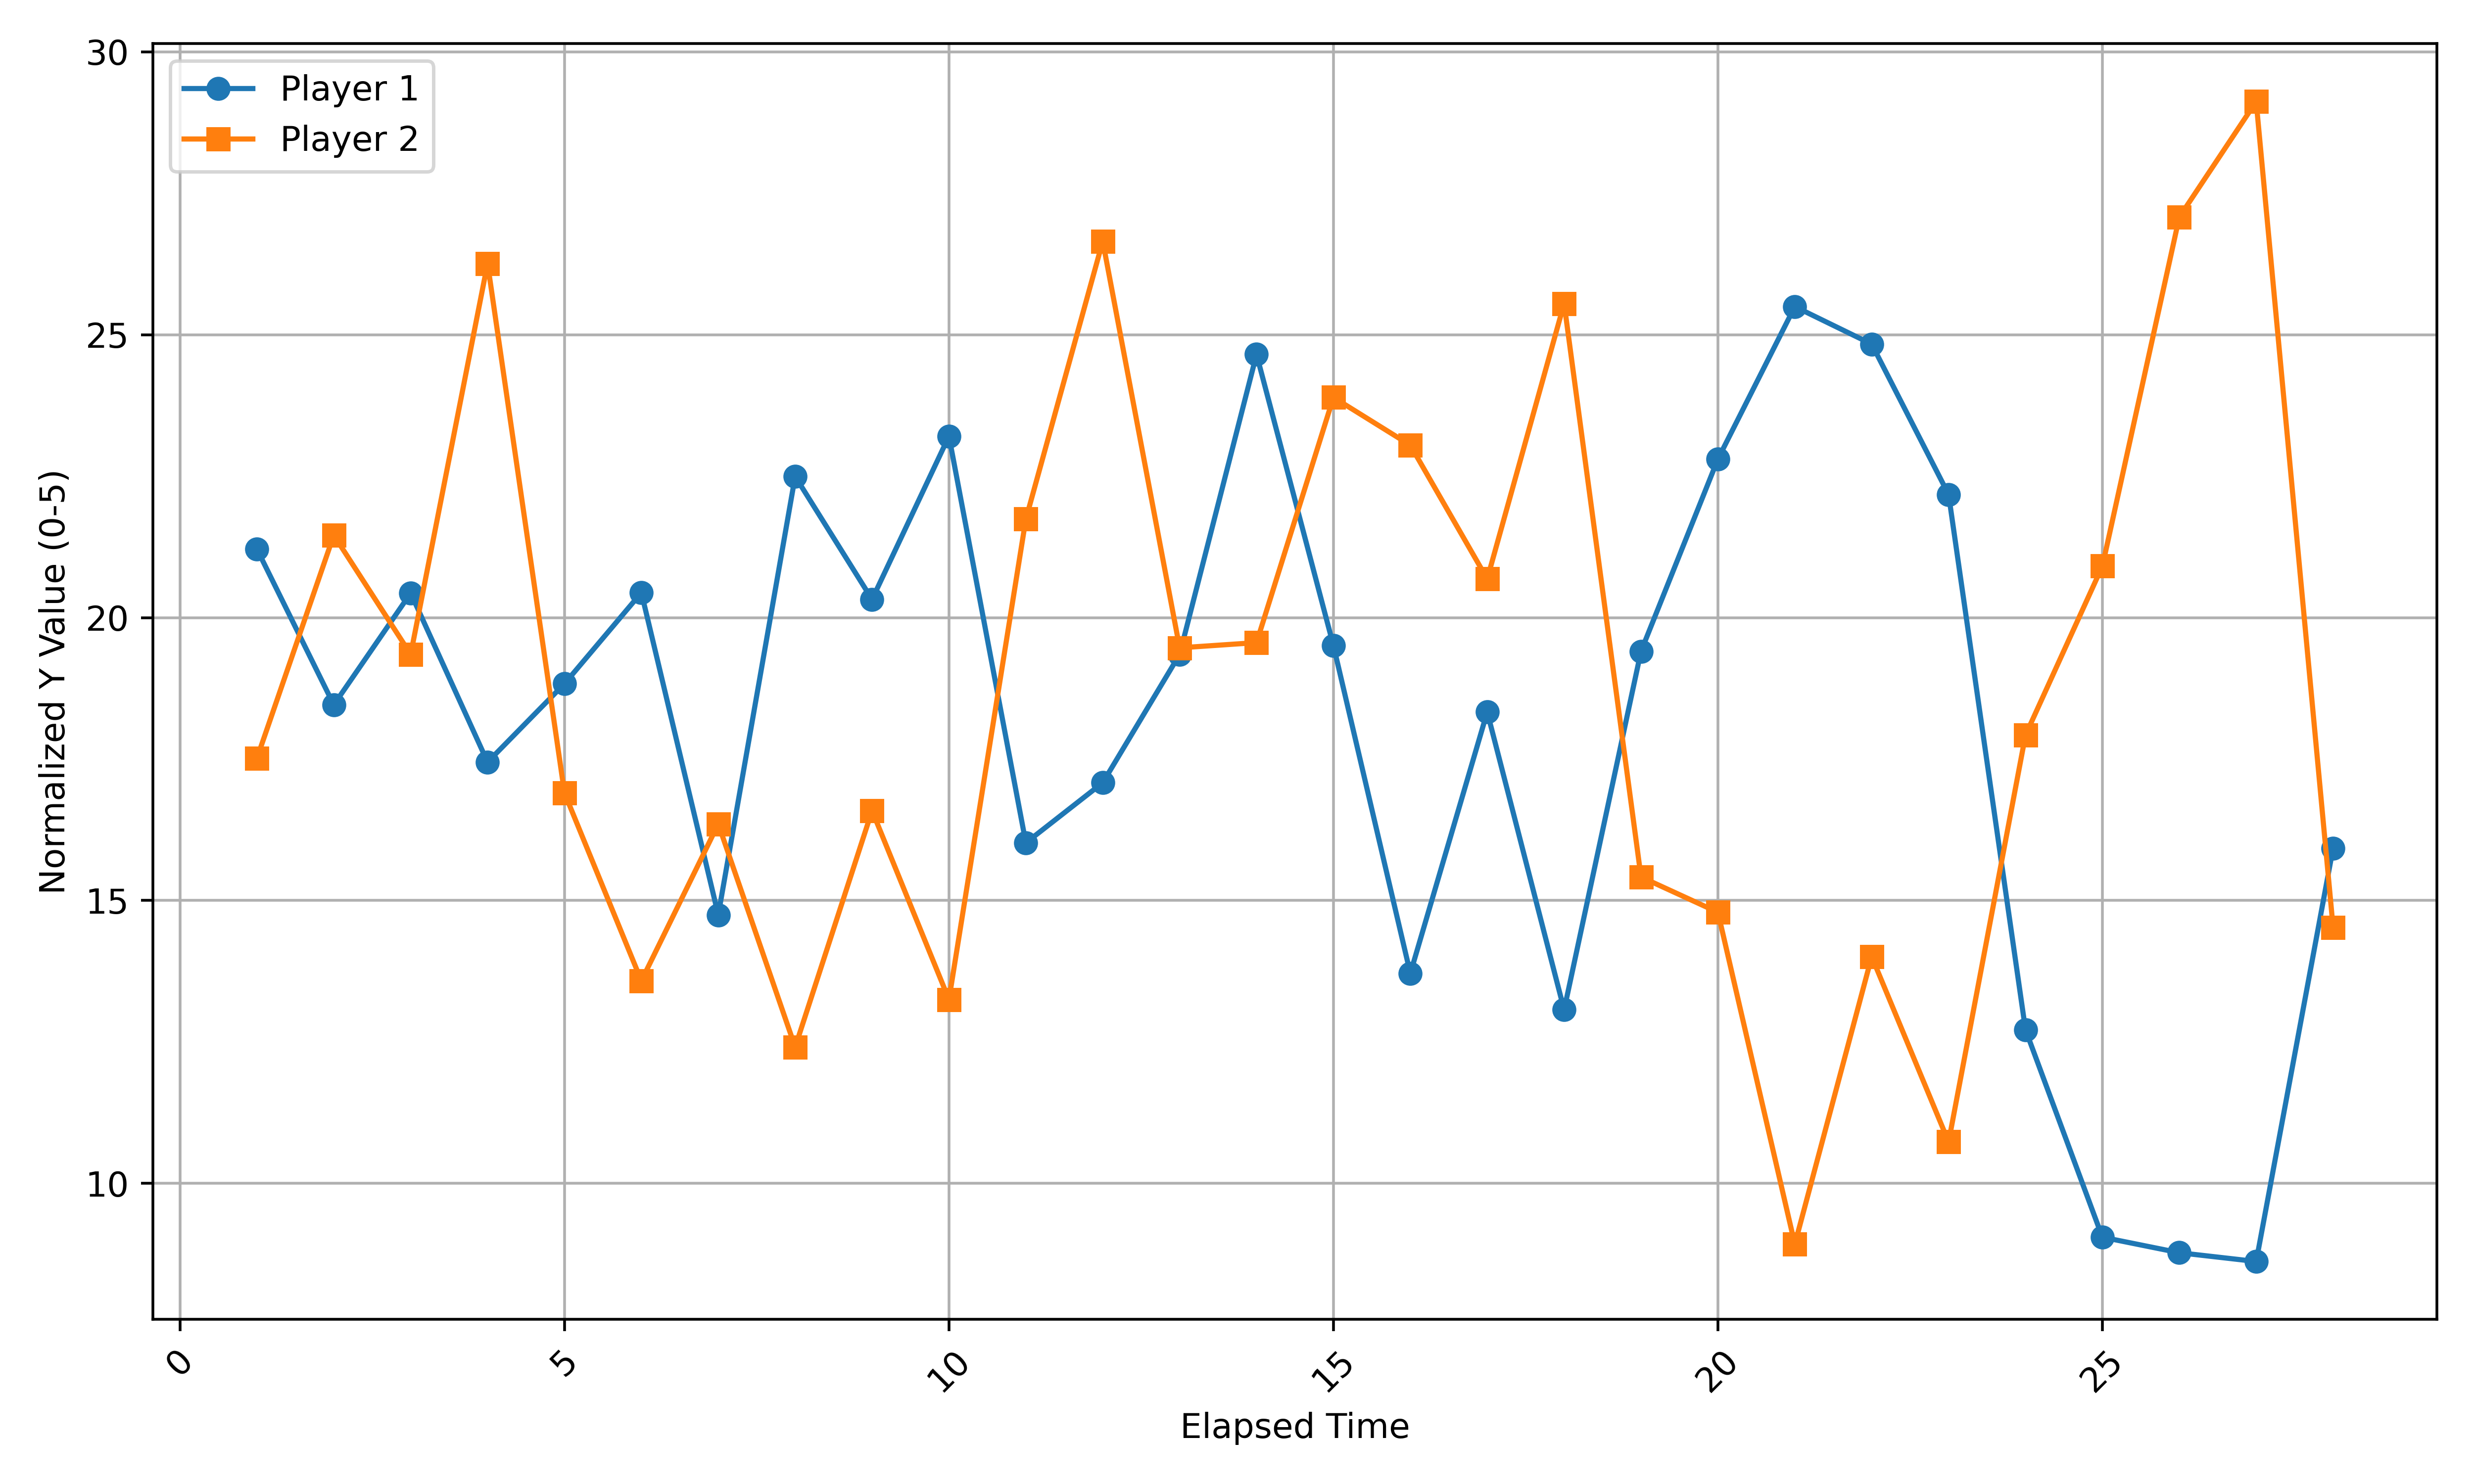
\includegraphics[width=\linewidth]{q11/动量_仅2人.png}
        \caption{Player momentum line chart}
        \label{fig_q11_2}
    \end{minipage}
\end{figure}


% 例如如果近几个回合的分差非常的大,那么拥有优势的一方往往会很自信,更有可能在未来的比分中将这种势头延续下去,从而将比分进一步的拉大。
% 这些玩家势头的波动就来自于不同特征值的一个变化,这个值的变化特别是带有时间滞后属性的值,更能反应球员现在的势头表现。
% 我们将比赛的比分的进行,还有玩家的势头整合进了一个表,旨在更加直观清晰的分辨出玩家势头对未来比赛得分的影响。
% 我们选取的数据是来自“2023\-wimbledon\-1301”场次的gmae\_no =1 set\_no = 1的前3局比赛。
% 在这些比赛场次中很好地反映了玩家在比分上的缠斗,逆转比分实现反超,以及统治全局取得压倒性胜利的各种情况。

For instance, if the score difference in recent rounds is significantly large, the advantaged side tends to be more confident and is more likely to continue this momentum in future scores, thereby further widening the score gap. These fluctuations in player momentum arise from changes in different feature values, especially those with time-lag attributes, which better reflect the current momentum performance of the player. We integrated the match scores and player momentum into Figure \ref{fig_q11_2}, aiming to more intuitively and clearly discern the impact of player momentum on future match scoring. The selected data comes from "game\_no" = 1 "set\_no" = 1 of the first three games of the "2023\-wimbledon\-1301" match. These matches well reflect the players' struggles in scoring, reversing scores for a comeback, and dominating the game for an overwhelming victory.

% 根据上述的目标,我们制作了图2。在第一局中,第二分时,玩家2在对手的发球局实现防守得分,从心理上还是从战术上都能证明去玩家2在那球表现的好,从而体现在势头的变化上。
% 玩家2的势头在第一球是还是比较低的水平,但是第一球成功防守后实现了对玩家1的反超。在第一局的第4个球开始,玩家的得分相出现了缠斗,在第八球时玩家1的势头明显高于是玩家2的势头,最终是由玩家1取得比赛的胜利。
% 第二局比赛则是玩家2的发球局,势头在决胜球前保持着玩家2优势的判断,同样最后是玩家2赢得了本场比赛。
% 随后的第三局和第四局则显示出了选手在自己的发球局取得压倒性胜利的情况,我们建立的势头模型显示出:在这种压倒性一方统治全局的比赛中,势头的差值会更大,并且在前几球就能达到比较大的差值。
% 这也能很好地说明该我们的Dynamic Momentum Index能很好地分析这种比赛的玩家们的表现。综上所诉我们建立的模型仅仅能反映出选手在当前时刻的状态,其当前势头状态和比赛结果走势符合,能较好地反应球员的运动状态。
Based on the aforementioned objectives, we created Figure \ref{fig_q11_1}. In the first game, at the second point, player 2 scores on defense during the opponent's service game, which psychologically and tactically proves player 2's superior performance in that rally, as reflected in the change in momentum. Player 2's momentum was relatively low at the first point, but after successfully defending the first ball, player 2 managed to overtake player 1. Starting with the fourth ball of the first game, the players' scores entangled, and by the eighth ball, player 1's momentum was clearly higher than player 2's, ultimately leading to player 1 winning the match. The second game was player 2's service game, with the momentum maintaining player 2's advantage up until the deciding point, and eventually, player 2 won the match. The third and fourth games then showed players achieving overwhelming victories in their service games, with our momentum model indicating that in such dominating matches, the difference in momentum would be greater, achieving significant differences in the initial points. This also effectively demonstrates that our Dynamic Momentum Index can accurately analyze the performance of players in such matches. In conclusion, our model merely reflects the players' current state, with the current momentum status and match outcome trends aligning well, effectively representing the athletes' physical states.
\subsection{Conclusion}
% 结论:我们有理由认为,在比赛中势头得分更高的球员在更有可能在后续的比赛得分中得分,势头差距越大这种概率越有可能发生,即我们可以说,势头分数越高的球员在赛场上表现越好。
We have reason to believe that in matches, players with higher momentum scores are more likely to score in subsequent games, and the greater the momentum difference, the more likely this probability occurs. Hence, we can say that players with higher momentum scores tend to perform better on the field.
cceshi
\section{Task 2: Determine if the swings and winning streaks in the match are random}
\subsection{Definition of Swings Points}:In the analysis of dynamic datasets, we define points signaling imminent trend shifts as change points, colloquially termed Swings points in the context of competitive sports.

Our methodology incorporates a time series change point detection model, leveraging the capabilities of the ruptures Python library. This library is distinguished for its offline change point detection functionalities, enabling the analysis and segmentation of non-stationary signals through both exact and approximate methods across diverse parametric and non-parametric models. ruptures is designed for user accessibility, offering a comprehensive, well-documented interface while also supporting modularity for the seamless integration and expansion of algorithms and models within its framework.
\subsection{Detection of Swings Points via Change Point Detection Model}:For the identification of Swings points, player momentum data, computed on a minute-by-minute basis, was inputted into the change point detection model to identify anomalies. These anomalies were subsequently annotated within the sequence data, with anomalous points being marked with a 1 and normal points with a 0. The annotated data was subjected to a test of randomness, the runs test, to assess the data's stochasticity.

A pass in this test indicates the data's randomness, suggesting the inaccuracy of coaches' intuitive judgments regarding game dynamics. In contrast, failure to pass the randomness test validates the precision of coaches' insights into the game's momentum shifts.
% \begin{\itemize}
% \item {\bf Swings检测}:
% \item {\bf 数据可视化}:
% \end{itemize}
\subsection{Winning Streaks and Swings Points Randomness Test}:Through data manipulation, we statistically assessed the occurrence of winning streaks for athlete A, paralleling the approach taken for Swings points detection. This involved the generation of a binary sequence, assigning a 1 for each instance of consecutive victories and a 0 for all other outcomes. Application of a randomness test to this sequence aimed to delineate the data's stochastic nature.
A pass in this test suggests that the observed patterns of winning streaks or Swings points are random, casting doubt on the accuracy of coaches' intuitions regarding game dynamics. Conversely, a failure in this test underscores the legitimacy of such intuitive insights, implying that these patterns are not purely coincidental and pose a challenge to the predictive capabilities of our momentum model.

\begin{itemize}
\item {\bf Introduction to the Runs Test}: The runs test serves as a non-parametric method for assessing the randomness within a sequence of binary data. It evaluates the sequence's arrangement by counting the runs, which are uninterrupted sequences of identical elements, to test the hypothesis of randomness. Deviations from the expected number of runs in a truly random sequence can signify non-randomness, providing insights into potential underlying patterns or predictability within the data.

\item {\bf Runs Test Analysis for Winning Streaks - Randomness Analysis}: Applying the runs test to the binary sequence of winning streaks allows us to scrutinize the randomness of these occurrences. The test evaluates whether the distribution of wins and losses among the athlete's performances deviates from randomness, thus gauging the predictability and efficacy of prevailing beliefs or models in forecasting outcomes based on historical performance data.
\begin{table}[ht]
    \centering
    \caption{Runs Test Results}
    \label{tab:runs_test_results}
    \begin{tabular}{lccc}
        \hline
        Name                 & Sample Size & \(z\)-value & \(P\)-value                                                               \\ \hline
        continuous\_wins\_p1 & 6201        & 2.069       & 0.039**                                                                   \\
        continuous\_wins\_p2 & 6201        & -0.377      & 0.706                                                                     \\ \hline
        \multicolumn{4}{l}{\footnotesize Note: ***, **, and * indicate significance at the 1\%, 5\%, and 10\% levels, respectively.} \\
    \end{tabular}
\end{table}

\item {\bf Swings Runs Test - Randomness Analysis}: The application of the runs test to the binary sequence denoting Swings points aims to discern whether these pivotal moments in gameplay are random occurrences or part of a discernible pattern. This analysis challenges the notion of random fluctuation in game momentum and tests the robustness of statistical models designed to predict such critical shifts.
\begin{table}[ht]
    \centering
    \caption{Runs Test Results for Turning Point Counts}
    \label{tab:runs_test_turning_points}
    \begin{tabular}{lccc}
        \hline
        Name                      & Sample Size & \(z\)-value & \(P\)-value                                                        \\ \hline
        p1\_Turning\_point\_count & 6196        & 17.253      & 0.000***                                                           \\
        p2\_Turning\_point\_count & 6196        & 17.296      & 0.000***                                                           \\ \hline
        \multicolumn{4}{l}{\footnotesize Note: ***, **, and * denote significance at the 1\%, 5\%, and 10\% levels, respectively.} \\
    \end{tabular}
\end{table}
\end{itemize}

% \subsection{Conclusion}
% The results of the runs tests applied to our dataset reveal significant insights into the randomness of the data associated with two variables: continuous_wins_p1 and continuous_wins_p2, as well as p1_Turning_point_count and p2_Turning_point_count. The significance levels indicated by the P-values from these tests are crucial for understanding the stochastic properties of the data, guiding the acceptance or rejection of our null hypothesis regarding data randomness.
% \begin{itemize}
%     \item For continuous\_wins\_p1 and p1\_Turning\_point\_count: The tests yielded P-values of 0.039** and 0.000***, respectively. Both outcomes are significant, with P-values less than 0.05, suggesting that the data for these variables is not random. Therefore, we reject the null hypothesis for these variables, indicating that the observed patterns are influenced by factors other than chance, suggesting a deterministic or predictable aspect in the data structure.
%     \item For continuous\_wins\_p2 and p2\_Turning\_point\_count: The P-value for continuous\_wins\_p2 was 0.706, indicating a lack of significance and suggesting that the data is random; hence, we cannot reject the null hypothesis for this variable. However, for p2\_Turning\_point\_count, the P-value was 0.000***, showing significant non-randomness, leading to the rejection of the null hypothesis similar to p1\_Turning\_point\_count.
% \end{itemize}


\quad~ We first give the value of parameters based on others’ studies. Then we get the calculation results and simulating results via those data.

\subsubsection{Determination of Parameters}

After establishing the model, we have to determine the value of some
important parameters.

As scholar Beum Kim points out, the optimal temperature for bath is
between 41 and 45$^\circ$C [1]. Meanwhile, according to Shimodozono's study, 41$^\circ$C warm water bath is the perfect choice for individual health [2]. So it is reasonable for us to focus on $41^\circ$C $\sim 45^\circ$C. Because adding hot water continuously is a steady process, so the mean temperature of bath water is supposed to be constant. We value the temperature of inflow and outflow water with the maximum and minimum temperature respectively.

The values of all parameters needed are shown as follows:

.....

\subsubsection{Calculating Results}

Putting the above value of parameters into the equations we derived before, we can get the some data as follows:


\section{Task 3}
\begin{figure}[!htb]
    \centering
    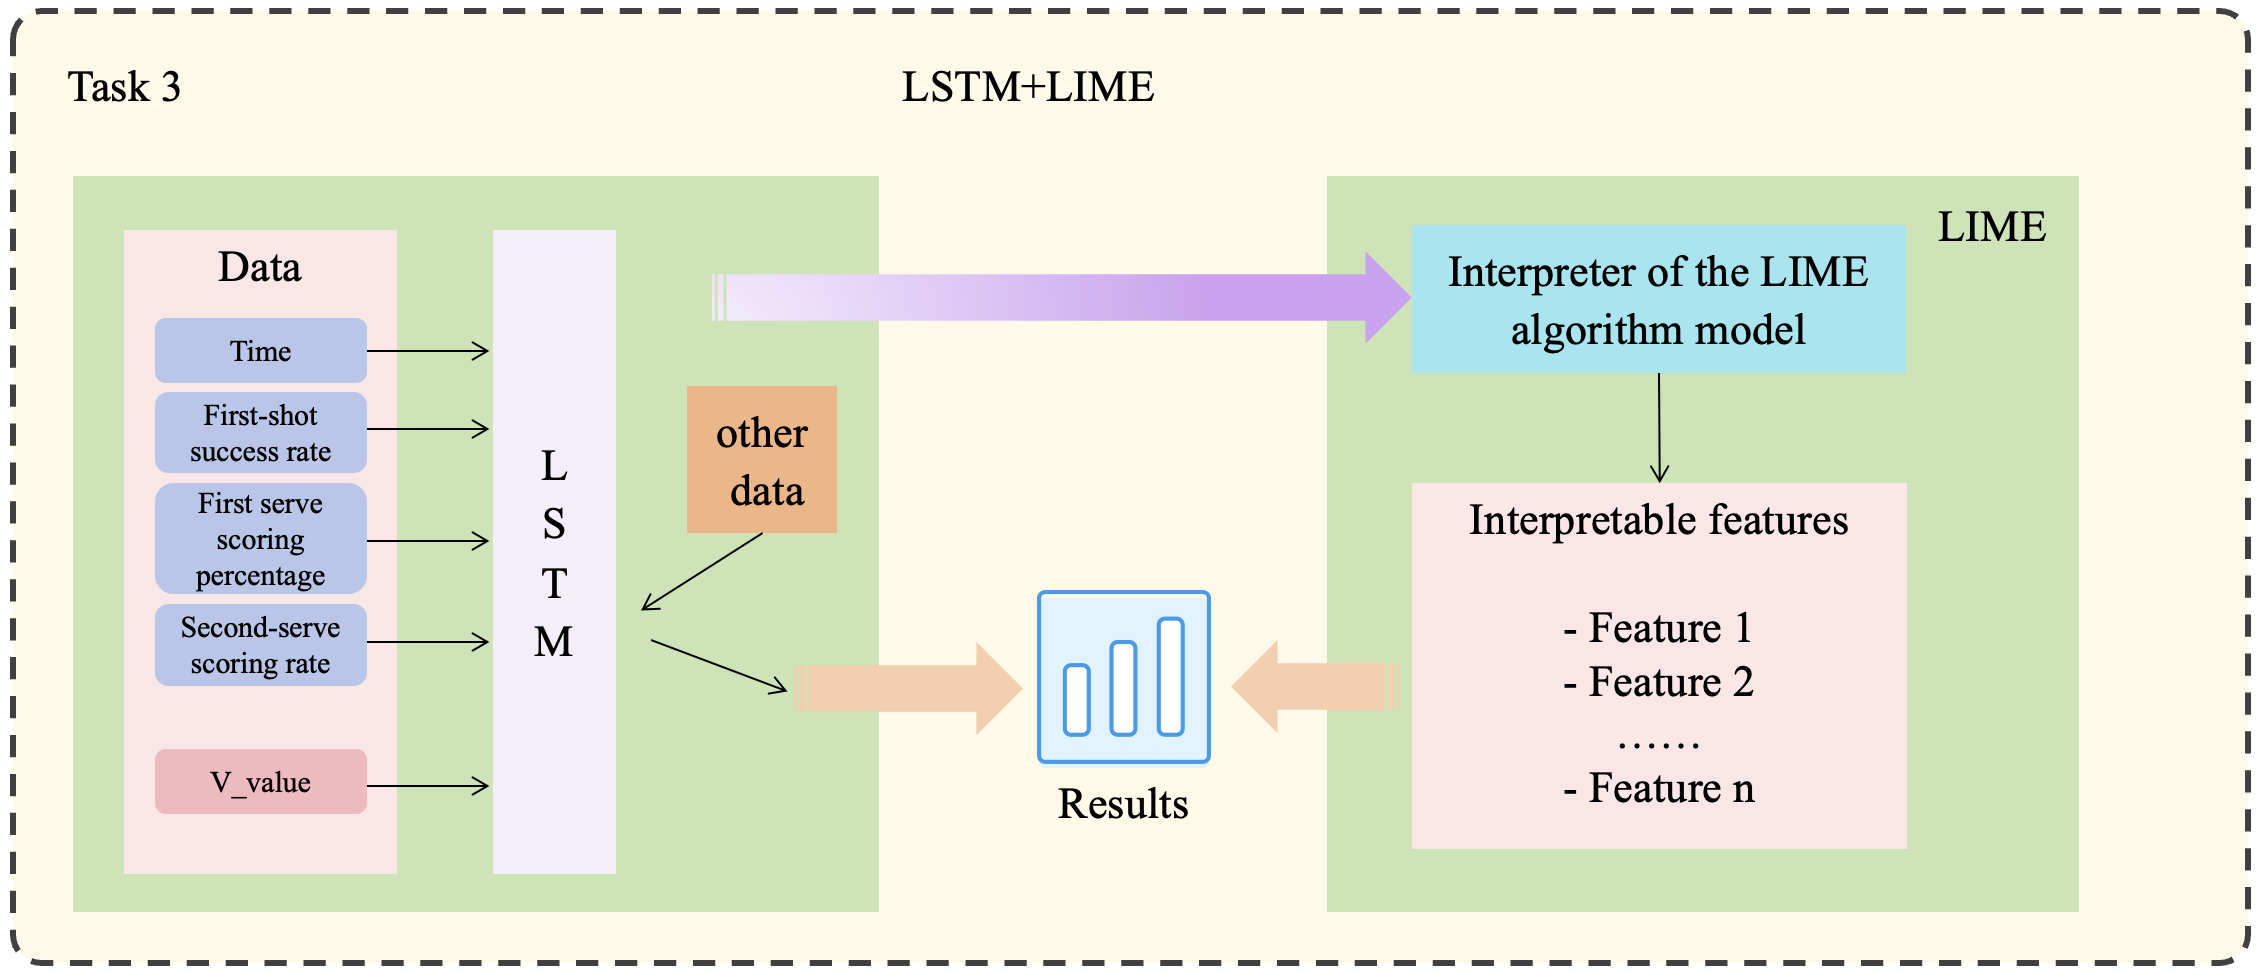
\includegraphics[width=16cm]{LSTM_LIME.png}
    \caption{Basic idea for task3} \label{fig:sample_value}
\end{figure}

Basic idea: use LSTM model to import features and predictors to predict the fluctuation of the game, and analyze which factors are most relevant by LIME model. Make recommendations to athletes based on the analyzed correlation metrics

\subsection{Predicting Athlete Momentum Using LSTM Models}

An LSTM model is used to analyze and predict momentum fluctuations during matches. LSTM is a time series prediction model that is particularly well suited for working with time-dependent data. In our application, this model is trained to capture and predict key turning points in tennis matches, i.e., changes in momentum of individual players during a match.

The match data is first preprocessed, including normalization and serialization, using \\''p1\_1st\_serve\_success\_ratio'', ''p1\_1st\_serve\_win\_ratio'', ''p1\_2nd\_serve\_win\_ratio'',\\ ''p1\_Players\_run\_distance\_difference'', ''p1\_server'', ''p1\_Player\_score\_margin'', which are the important factors filtered out from the total model statistics of the first question, are used as the eigenvalues to predict ``y\_value\_p1\_normalized\_0\_5'' as the predicted value.

After model training, we obtained the following data and visualization images:
\begin{figure}[!ht]
    \centering
    \begin{minipage}{0.40\textwidth}
        \centering
        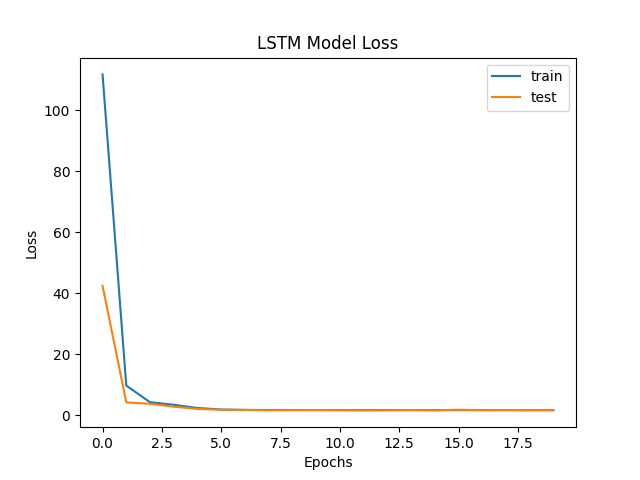
\includegraphics[width=\linewidth]{Epochs_Loss.png} % 将width调整为适合minipage宽度的大小
        \caption{Modeling process}
        \label{fig:epochs_loss}
    \end{minipage}\hfill % \hfill用于在两个minipage之间添加空白,使它们分布在页面的两侧
    \begin{minipage}{0.45\textwidth}
        \centering
        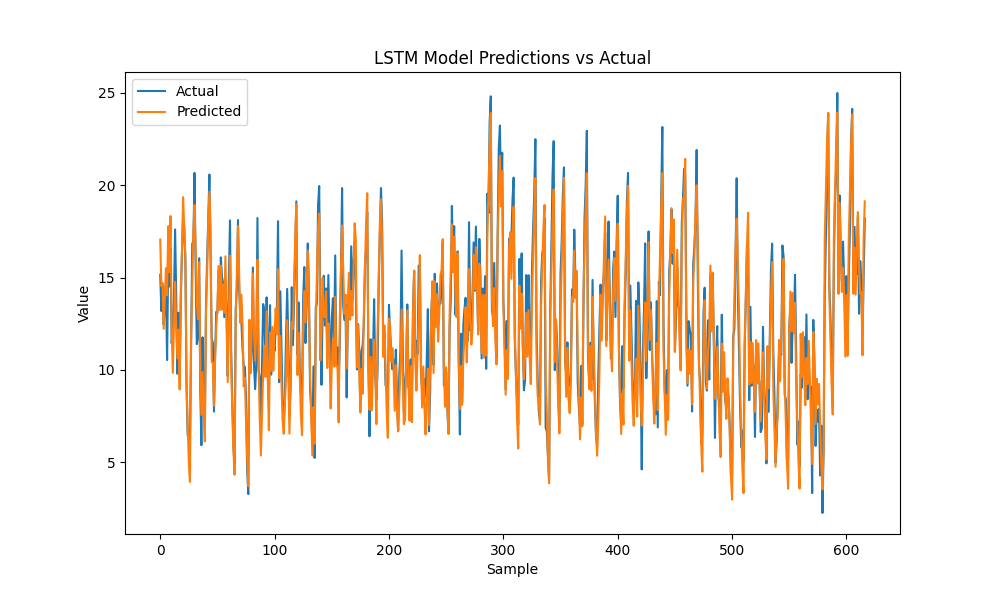
\includegraphics[width=\linewidth]{Sample_Value.png} % 同样,调整width以适应minipage
        \caption{Predicted \& Actual Values}
        \label{fig:sample_value}
    \end{minipage}
\end{figure}


Mean Absolute Error: 1.0477484090257072

Mean Squared Error: 1.6303017250768546

Root Mean Squared Error: 1.2768326926723228



% \begin{figure}[!htb]
%     \centering
%     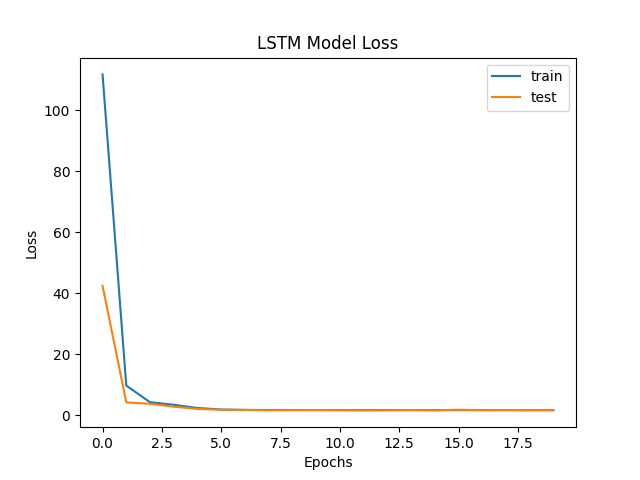
\includegraphics[width=8cm]{Epochs_Loss.png}
%     \caption{Modeling process} \label{fig:epochs_loss}
% \end{figure}

% \begin{figure}[!htb]
%     \centering
%     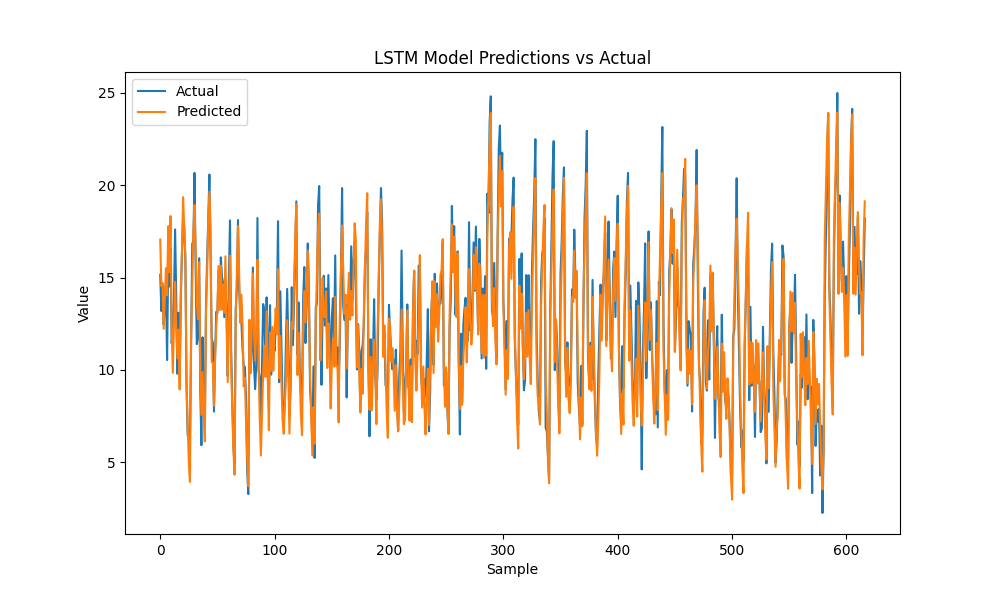
\includegraphics[width=8cm]{Sample_Value.png}
%     \caption{Predicted vs Actual Values} \label{fig:sample_value}
% \end{figure}

Among other things, it can be seen from the LSTM model performance graph that the loss of the model on the training and test sets decreases with the increase of the training period, which means that the predictive ability of the model improves with time. From the performance metrics, Mean Absolute Error, MAE is 1.0477, Mean Squared Error, MSE is 1.6303, and Root Mean Squared Error is 1.2768.These metrics show that the model has some prediction accuracy, especially the low MAE and RMSE, which indicates that the model prediction results are closer to the actual data.

The above data show that the model has good prediction performance.


\subsection{LIME and Advice for Athletes}

LSTM is a time series prediction model that is particularly well suited for working with time-dependent data. In our application, this model is trained to identify and predict key turning points in a tennis match, i.e., changes in the momentum of the match.The LIME model provides us with a way to interpret the predictions of a complex model. With LIME, we can identify which features are most important for predicting momentum changes.

\begin{figure}[!htb]
    \centering
    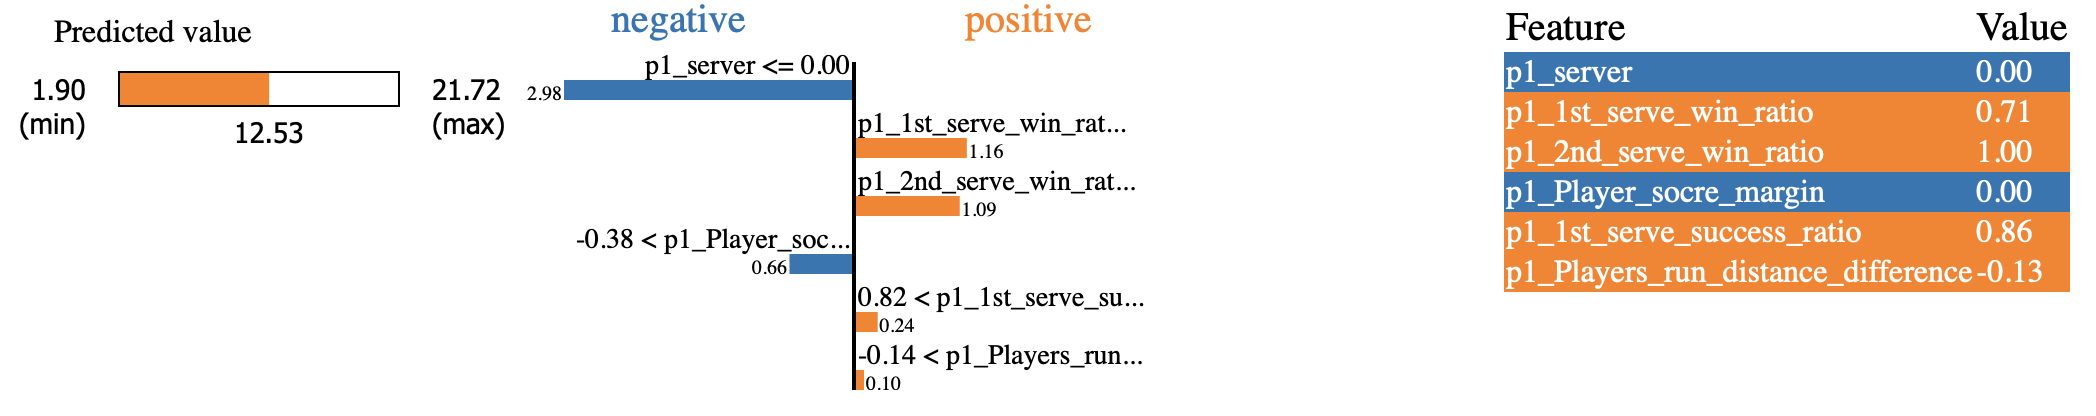
\includegraphics[width=16cm]{LIME.png}
    \caption{LIME Results} \label{fig:sample_value}
\end{figure}

% \subsection{Advice for Athletes}
With an understanding of the key factors predicted by the model, we can develop targeted strategies for athletes.

\begin{itemize}
    \item[] {\bf Increase first-shot scoring}: Given that first serve percentage is a key factor in the momentum of a match, athletes need to improve this metric through technical and strategic training. This may include enhancing serve speed and accuracy, as well as experimenting with different angles and spins on the serve.

    \item[] {\bf Optimize second shot scoring rate}: Second serve percentage also has a significant impact on momentum, and athletes should ensure that second serves are safe and effective when first serves are not scored. This may mean choosing a more conservative second serve strategy when first serves are not scored, or training to maintain a consistent second serve under pressure.

    \item[] {\bf Controlling the pace of the game}:The results of the LIME model also show that running distance differences have an impact on momentum. Athletes should control the pace of the match by improving their positional sense and tactical awareness to minimize their movement and make their opponents work harder

    \item[] {\bf Comprehensive training and strategy adjustment}: Athletes need to combine the results of these analyses with comprehensive training to optimize their performance in matches. In addition, strategy adjustments may need to be made for the specifics of different opponents.

\end{itemize}
Through the above model analysis and strategy suggestions, we can help athletes better understand the change of momentum in the game and provide scientific data support for them in future games. In practical applications, this combination of modeling and strategy can significantly improve the athletes' level of play and chances of winning.

\section{Task 4}
Advising players to prepare for new matches against different opponents :

In order to advise players to prepare for matches against different opponents, we recommend using historical match data and adapting the model to the characteristics of the new opponent by retraining it. This includes collecting past match data, technical statistics, and playing styles of the new opponent. By testing the model on one or more other matches, the model's performance in the new opponent scenario can be evaluated and adjustments can be made.

How accurate is the model in predicting turnovers in matches?

The accuracy of the model in predicting turns in a match can be assessed by comparing the model's predictions with actual match results. This can be done by reviewing historical matches and comparing them to the model's predictions. If the model performs poorly at certain times, this can be done by analyzing the sources of error in the model and identifying additional factors that may need to be included. If the model performs poorly at certain times, a feature importance analysis can be performed to identify the metrics that have the greatest impact on the model's performance. This helps to identify the weak points of the model in specific contexts. Further, more relevant features can be introduced by performing metric derivation for important metrics to improve the generalization of the model.

Model generalizability.

Our model has a wide range of adaptability, which is mainly due to the diversity and adequacy of the training data we choose. By using a large amount of data contest data, we ensure that the model is able to learn and understand the generalized patterns and trends behind various contests. We focus on capturing the full picture of key metrics, and strengthen the model's understanding of key factors through feature importance analysis and metric derivation. This design approach allows the model to perform well against different opponents, game types, and even other sports. We are constantly evaluating and updating the model to ensure its adaptability and continued superior performance. As a result, we are confident that our models have a high degree of generalizability and are able to effectively address a wide range of challenges in different environments.

In order to improve the generalizability of the model, the model performance is continuously monitored in new domains or scenarios in future studies, and adjustments and updates are made based on actual performance.

\section{Model Analysis and Sensitivity Analysis}

In this investigation, we examine the impact of enhancing the serve weight on the predictive performance of a Long Short-Term Memory (LSTM) model, utilizing a sophisticatedly simulated dataset. Our methodology extends beyond mere weight adjustment of the serve feature; it encompasses a comprehensive sensitivity analysis that meticulously evaluates its influence on predicting match outcomes. The introduction of noise perturbations aims to simulate real-world data variability, thereby ensuring the robustness of our findings. Despite the increased complexity introduced by these perturbations, our analysis unveils a consistent pattern: model performance improves with an increase in serve weight up to a specific threshold, beyond which it experiences a decline. This pattern underscores the critical balance required in feature weighting within predictive models, highlighting the danger of over-reliance on a singular feature for prediction accuracy.

% Uncomment the following lines and replace "example-image.jpg" with your actual image file name
\begin{figure}[htbp]
    \centering
    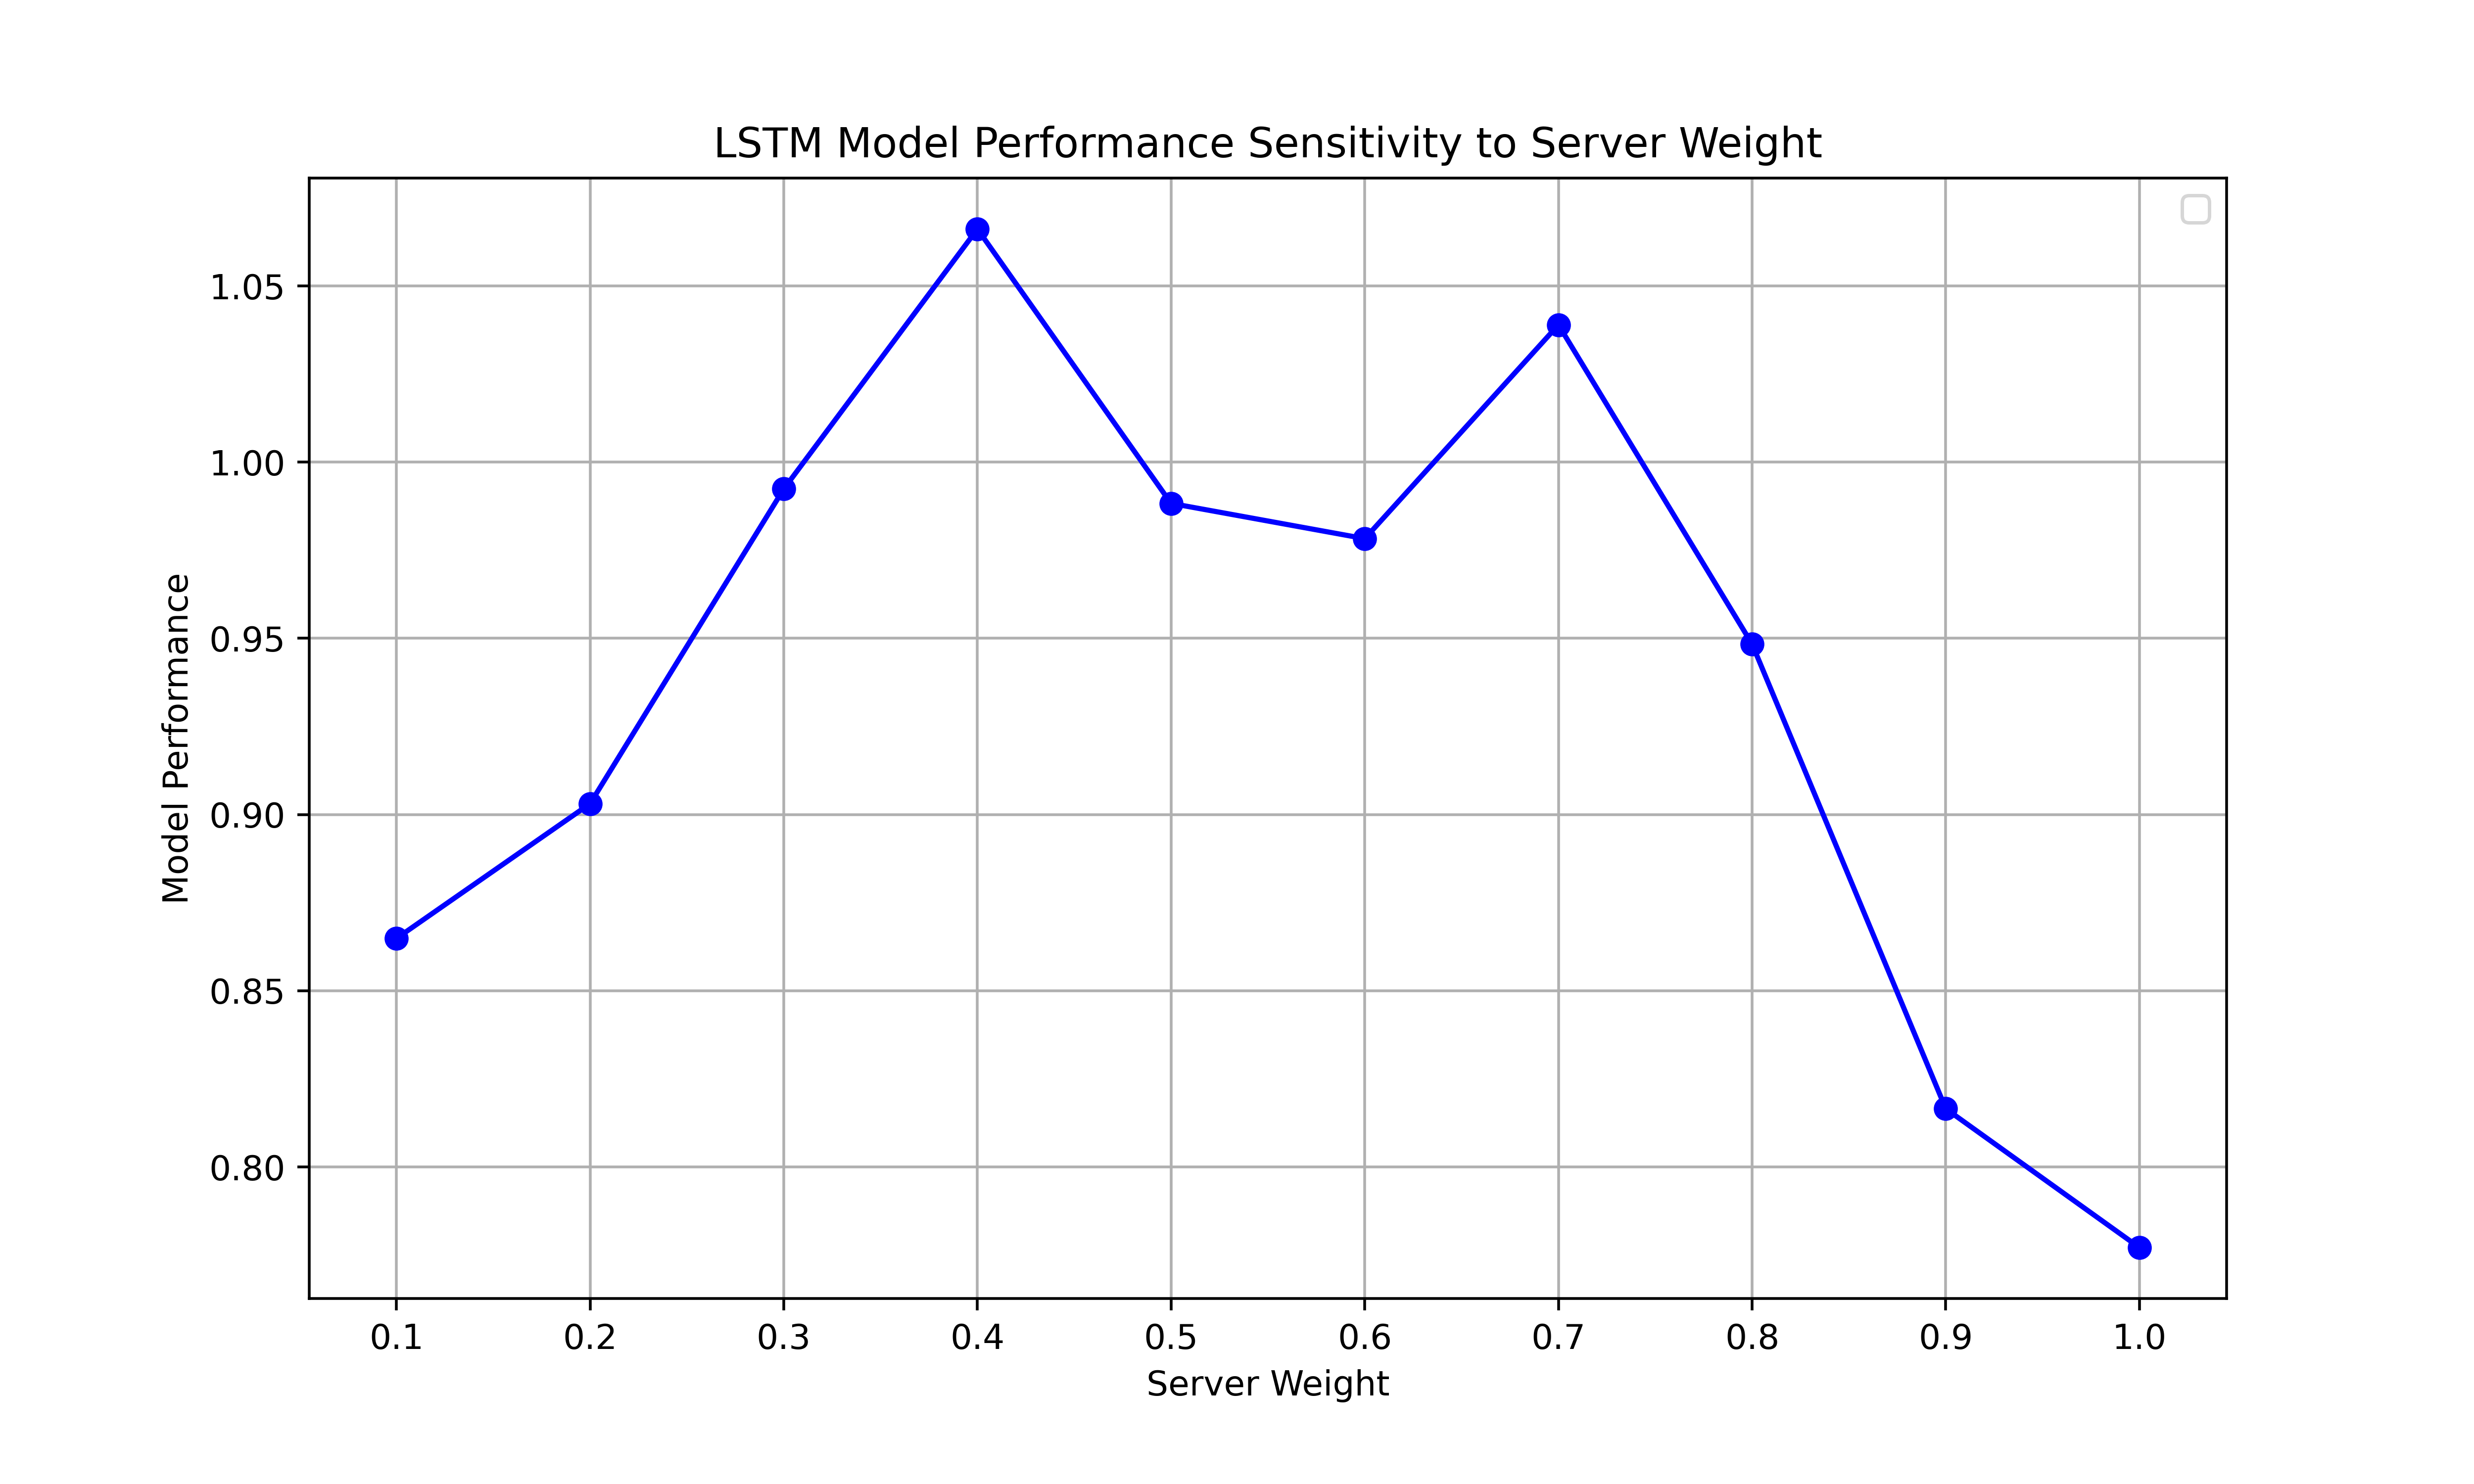
\includegraphics[width=0.8\textwidth]{Sensitivity Analysis.jpg} % 图片文件名和路径
    % \caption{这是一张示例图片} % 图片标题
    \label{fig:example} % 用于文内引用的标签
\end{figure}

While our model employs an advanced framework capable of capturing the intricate dynamics of match outcomes, it's important to note that our findings, though based on simulated data, are crafted to mirror the nuances of real-world scenarios closely. The introduction of noise and the careful adjustment of feature weights reflect a deliberate effort to enhance the model's applicability and reliability in practical settings. This study's insights, underscored by a rigorous sensitivity analysis, not only shed light on the optimal utilization of serve weight in predictive models but also emphasize the importance of detailed analysis in the development of robust sports analytics tools. Our work contributes to the broader discourse in sports analytics, advocating for a nuanced and balanced approach to model development and refinement.

% \subsubsection{Different Volumes of Bathtubs}

% In reality, a cup of water will be cooled down rapidly. However, it takes quite long time for a bucket of water to become cool. That is because their volume is different and the specific heat of water is very large. So that the decrease of temperature is not obvious if the volume of water is huge. That also explains why it takes 45 min for 320 L water to be cooled by 1$^\circ$C.

% In order to examine the influence of volume, we analyze our sub-models
% by conducting sensitivity Analysis to them.

% We assume the initial volume to be 280 L and change it by $\pm 5$\%, $\pm 8$\%, $\pm 12$\% and $\pm 15$\%. With the aid of sub-models we established before, the variation of some parameters turns out to be as follows

%%三线表


\section{Strength and Weakness}

\subsection{Strength}

\begin{itemize}
    \item[] {\bf Comprehensive Analysis}: The approach taken to analyze player momentum and game outcomes is thorough and multifaceted, integrating statistical analysis, machine learning models, and sensitivity analysis. This comprehensive approach allows for a nuanced understanding of the factors that influence match dynamics.

    \item[] {\bf Innovative Use of Technology}: ploying advanced analytical techniques such as LSTM and LIME for predictive modeling and feature importance analysis, the study leverages cutting-edge technology to offer novel insights into sports analytics.

    \item[] {\bf Practical Recommendations}: The study provides actionable advice for athletes, focusing on areas like serve improvement and game pace control. These recommendations are directly derived from the model's findings, making them specifically tailored to enhancing athletic performance.

    \item[] {\bf Adaptability of the Model}: The inclusion of sensitivity analysis and the model's demonstrated ability to adapt to different opponents and match conditions showcase its flexibility. This adaptability is crucial for its application across various match scenarios and sports.

\end{itemize}

\subsection{Weakness}

\begin{itemize}
    \item[] {\bf Simulated Data Limitations}: While the model is designed to reflect real-world scenarios closely, the reliance on simulated data for some analyses may not capture all the complexities of actual matches. This could limit the model's accuracy in predicting real-world outcomes.

    \item[] {\bf Feature Weighting Challenges}: The sensitivity analysis reveals that the model's performance is highly dependent on the precise weighting of features such as the serve. Determining the optimal balance of feature weights can be challenging and may require extensive tuning.

    \item[] {\bf Potential Overfitting}:  While not explicitly mentioned, the intricate nature of the model and the use of multiple machine learning techniques raise concerns about overfitting. Ensuring the model's generalizability to unseen data is crucial for its effectiveness in real-world applications.

\end{itemize}

\section{Further Discussion}

Given that our model and work is not yet complete, we hope to complete a more comprehensive mathematical model with more in-depth research. So far, our team's understanding of the background of the sport of tennis and the application of multiple models to the sport has been insufficient. We very much hope to make our model more complete through a deeper understanding of the relevant background knowledge. For example, we can add more factors that affect athletes' momentum to our model to make our predictions more accurate. As we mentioned before, research on analyzing and coaching tennis is significant, so we will try our best to do more research to improve the performance of our model.


\begin{thebibliography}{99}
    \addcontentsline{toc}{section}{Reference}

    \bibitem{1} Noel, J. T. P., Da Fonseca, V. P., \& Soares, A. (2024). A Comprehensive Data Pipeline for Comparing the Effects of Momentum on Sports Leagues. Data, 9(2), 29. https://doi.org/10.3390/data9020029
    \bibitem{2} Covassin, T. M. (1999). The relationship between psychosocial momentum, precipitating events, and tennis match outcome. University of Nevada, Las Vegas.
    \bibitem{3} Dietl, H., \& Nesseler, C. (2017). Momentum in tennis: Controlling the match. UZH Business Working Paper Series, (365).
    \bibitem{4} Ma, Jia-Cai, Chen, Q. K., Liang, C. R., \& Zhou, Z. C.. (2023). Modeling and research analysis of match-winning factors of professional tennis players. Bulletin of Sports Science and Technology Literature, 31(4), 66-68.(In Chinese)

\end{thebibliography}

\newpage

\begin{letter}{What impact does a tennis player's "potential energy" have on the game?}
    In this study, we aimed to explore how tennis players' potential energy affects the outcome of the game by building a mathematical model. We focus on data from a single game and try to predict an athlete's future "momentum" performance. Using a series of mathematical models, we investigated how changes in potential energy affect an athlete's overall performance during competition.

    We first developed a potential energy calculation model that took into account factors such as the athlete's physical strength, skill level, and field conditions. This model is based on actual game data to more accurately reflect the status of athletes during the game. We analyzed data from multiple games to verify the accuracy and practicality of our mathematical model. By comparing actual match results with model predictions, we are able to derive the exact impact of potential energy on match outcomes.

    Through this study, we discovered that an athlete's potential energy does indeed play a key role in competition. Our mathematical model not only provides an in-depth understanding of potential energy changes, but also successfully predicts future momentum trends for athletes. This provides coaches and athletes with a powerful tool to optimize training and competition strategies.

    We hope to further expand this model in the future to consider more influencing factors, such as psychological state, opponent level, etc. This will help improve our understanding of athlete performance and provide more accurate guidance for individualized training.

    By reading our research model, I believe you will gain a new understanding of the concept of "potential energy" and be able to apply it to actual tennis matches. Our research not only enriches the understanding of kinetic energy changes in tennis matches, but also provides new ideas and methods for future tennis match research.
\end{letter}

\newpage

\begin{appendices}

    \section{First appendix}

    Here are simulation programmes we used in our model as follow.\\

    \textbf{\textcolor[rgb]{0.98,0.00,0.00}{Input PYTHON source:}}
    \lstinputlisting[language=PYTHON]{/Users/zeyu/Documents/Learning/数学建模/美赛数学建模/git/comap_mcm_2024/Code/Q1/putcodeonpage.py}

    \section{Second appendix}

    some more text \textcolor[rgb]{0.98,0.00,0.00}{\textbf{Input PYTHON source:}}
    \lstinputlisting[language=python]{/Users/zeyu/Documents/Learning/数学建模/美赛数学建模/git/comap_mcm_2024/Code/Q3/code/LSTM+LIME.py}

\end{appendices}
\end{document}
